\documentclass{article}

% NeurIPS 2026 style, review mode (no options = anonymous, line numbers).
\usepackage{neurips_2026}

\usepackage{amsmath, amssymb, amsthm}
\usepackage{booktabs}
\usepackage[colorlinks=true, linkcolor=blue, citecolor=blue, urlcolor=blue]{hyperref}
\usepackage{graphicx}
\usepackage{xcolor}
\usepackage{algorithm}
\usepackage{algpseudocode}
\usepackage{natbib}
\usepackage{microtype}

% EDGE modifications to the base SAC algorithm are colored blue in
% Algorithm 1 to make the diff readable at a glance.
\definecolor{edgeblue}{HTML}{1F5AB5}
\newcommand{\edgemod}[1]{\textcolor{edgeblue}{#1}}

% Expert-normalized advantage. Defined once in the Evaluation Protocol
% (Section~\ref{sec:protocol}) and used everywhere afterwards.
% Numerator: per-seed return minus expert reference $J_{\mathrm{exp}}$.
% Denominator: $J_{\mathrm{ref}} - J_{\mathrm{exp}}$, where
% $J_{\mathrm{ref}}$ is a fixed task-specific reference scale chosen
% without reference to any method evaluated in this paper.
% Sign convention: $\tilde\Delta=0$ matches the expert, $\tilde\Delta=1$
% matches the reference scale, $\tilde\Delta<0$ underperforms.
\newcommand{\nbias}{\tilde{\Delta}}

\newtheorem{proposition}{Proposition}
\newtheorem{theorem}{Theorem}
\newtheorem{lemma}{Lemma}
\newtheorem{corollary}{Corollary}
\newtheorem{definition}{Definition}
\newtheorem{remark}{Remark}

% ============================================================
% PAPER METADATA
% ============================================================

\title{When (and How) to Trust the Expert: Diagnosing Query-Time Expert-Guided Reinforcement Learning}

\author{%
  Anonymous Author(s) \\
  Affiliation \\
  Address \\
  \texttt{email} \\
}

\begin{document}
\maketitle

% ============================================================
\begin{abstract}
% ============================================================

Many continuous-control problems come with a competent but
suboptimal off-the-shelf controller (a tuned PID, a hand-designed
gait), and a growing family of methods uses them as queryable
experts during reinforcement learning. These methods have been
proposed across separate papers without a common protocol or
imperfect-expert testing. We assemble the comparison on a shared
SAC backbone, restricted to query-time-controller
methods (IBRL, two JSRL variants, Residual SAC), and introduce a fifth
design point: \textbf{Expert-Driven Guided Exploration (EDGE)}, a
softmax over ensemble \emph{lower-confidence-bound} critic values
with gating form and pessimism ablated separately. Empirically,
EDGE is co-best with JSRL-curriculum under expert-action-noise
degradation ($13\%$ worst-case gap to per-task best vs.\
$\ge 21\%$ for the other methods) but trails on clean evaluation:
the asymptote-vs-robustness tradeoff this exposes is itself a
finding. Methods share a common HPO and evaluation protocol with
$100/50$ seeds on control/locomotion tasks; an action-noise sweep
(Gaussian jitter at three intensities) supplements the clean
evaluation. The benchmark surfaces three mechanism-specific failure modes.
\textbf{(F1) Critic blind spot under argmax-plus-bootstrap:} IBRL
is dominated by no-expert SAC on FourTank, our most
near-ceiling-expert task. \textbf{(F2) Residual saturation when the
expert is far from optimal:} Residual SAC's clean gap to per-task
best ranges from $0\%$ on FourTank (near-optimal PID) to $64\%$ on
Plane3DCircle (weak PID). \textbf{(F3) Warm-start buffer poisoning
under training-time handoff:} the training-time JSRL variant loses
$79\%$ of its clean return on CheetahRun and reverses sign on
Plane3DCircle under moderate action-noise jitter. We close with a candidate decision
rule keyed on three pre-training observables (expert quality, task
termination, expected deployment perturbation), framed as a
hypothesis to test. Code, hyperparameters, and results released.


\end{abstract}

% ============================================================
\section{Introduction}
% ============================================================

Many continuous-control problems come equipped with a queryable expert
policy: a hand-engineered feedback controller (PID, LQR, MPC), a motion
planner, a pattern generator, or a behaviorally-cloned demonstrator.
Such experts are rarely optimal but typically far better than a random
policy, and they encode knowledge that would be expensive to rediscover
from scratch. Most expert-guided RL papers (DAgger
\citep{ross2011dagger}, AWAC \citep{nair2020awac}, IBRL
\citep{hu2023ibrl}, RLPD \citep{ball2023rlpd}) treat the expert as an
upper bound: the goal is to match it. We study the complementary
question: given a controller already running on the plant, can we train
an RL policy that \emph{exceeds} its performance? The concrete
criterion throughout the paper is that a method must beat both the
RL-only baseline and the expert controller simultaneously.

\textbf{Contributions.}
\begin{itemize}
\item A surpass-the-expert benchmark of five expert-guided methods
(IBRL, two JSRL variants, Residual SAC, EDGE) on six tasks, common
HPO and base learner, with an expert action-noise degradation sweep.
\item A task-structural decision rule (Section~\ref{sec:when-to-use})
mapping termination, expert-quality, and incrementality to method
choice.
\item Three findings that contradict standard expectation: the
asymptote-strongest baseline (JSRL-training-time) is the
degradation-weakest; Residual SAC dominates a specific niche;
IBRL's argmax bootstrap drags the policy below the no-expert
baseline on near-ceiling experts (FourTank: pre-registered
one-sided permutation test, $p = 0.034$).
\item EDGE, a quality-aware ensemble-pessimism-gated mixing method
designed to avoid the IBRL blind spot
(Remark~\ref{rem:blindspot}). Empirically competitive on every
task and uniquely robust under expert degradation; the recommended
default whenever expert quality at deploy is uncertain.
\item Falsification protocol (buffer-coverage tests, ablations) in
Appendices~\ref{app:exploration},~\ref{app:ablation}.
\end{itemize}

% ============================================================
\section{Problem Formalization}
\label{sec:problem}
% ============================================================

We consider a continuous-control MDP
$(\mathcal{S}, \mathcal{A}, T, R, \gamma)$ with state space
$\mathcal{S} \subseteq \mathbb{R}^n$, action space $\mathcal{A} = [-1,1]^d$,
transition function $T: \mathcal{S} \times \mathcal{A} \to \mathcal{S}$, and
reward $R: \mathcal{S} \times \mathcal{A} \to \mathbb{R}$. Alongside the MDP
we are given a deterministic \emph{expert controller} $\pi^* : \mathcal{S}
\to \mathcal{A}$, typically a hand-engineered PID, LQR, MPC, or pattern
generator, that can be queried at any state visited during training. The
expert is not assumed to be optimal: we evaluate against it as a floor,
not as a target.

The agent's objective is the standard
$J(\pi) = \mathbb{E}\left[\sum_{t=0}^\infty \gamma^t R(s_t, a_t)\right]$.
We denote the expert's return as $J_{\text{exp}}$ and the RL-only
baseline's return at convergence as $J_{\text{RL}}$. We also fix a
task-specific reference scale $J_{\mathrm{ref}}$ used to
expert-normalize returns across tasks (defined in
Section~\ref{sec:protocol}). Our evaluation criterion is that a
candidate method must \emph{simultaneously} exceed both
$J_{\text{exp}}$ and $J_{\text{RL}}$ on every task where either
baseline leaves measurable headroom.

\paragraph{Expert-mixed behavior policy.}
EDGE acts under an expert-mixed behavior policy with a
\emph{quality-aware} gate: at each step, the gate probability is set
from a comparison of \emph{ensemble-pessimistic Q-estimates} at the
expert and policy actions, and the executed action is sampled from
\begin{equation}
    \beta_t(a\mid s) \;=\; p_t(s)\,\delta_{\pi^*(s)}(a)
    \;+\;(1-p_t(s))\,\pi_\theta(a\mid s),
    \quad
    p_t(s) \;=\; \sigma\!\Big(\tfrac{\check{Q}_t(s,\pi^*(s)) -
                              \check{Q}_t(s,\pi_\theta(s))}{\tau}\Big),
    \label{eq:behavior}
\end{equation}
where $\check{Q}_t(s,a) = Q^{\min}_\phi(s,a) - \beta\,(Q^{\max}_\phi(s,a)
- Q^{\min}_\phi(s,a))$ is the ensemble-pessimistic Q-estimate (the
critic-ensemble minimum, further penalized by ensemble spread), $\tau$
is a temperature, and $\sigma$ is the logistic. The replay buffer
stores $(s, a, r, s')$ tuples with $a \sim \beta_t$, and is consumed by
any off-policy RL algorithm that tolerates arbitrary full-support
behavior policies (e.g.\ SAC). Crucially, $0 < p_t(s) < 1$ at every
state with non-degenerate critic disagreement, so the gate preserves
full support over both arms.


% ============================================================
\section{Related Work}
% ============================================================

Expert-guided RL methods place along three axes: argmax selection
(IBRL \citep{hu2023ibrl}), training-time handoff (JSRL
\citep{uchendu2023jsrl} curriculum and warm-start variants), and
additive correction (Residual SAC
\citep{johannink2019residual}). Our comparison is restricted to
methods that consume the expert as a query-time policy at every
state. Policy-prior and offline-demonstration methods (DAgger
\citep{ross2011dagger}, AWAC \citep{nair2020awac}, PEX
\citep{zhang2023pex}, LOGO \citep{rengarajan2022logo}) and
static-buffer methods (RLPD \citep{ball2023rlpd}, IQL
\citep{kostrikov2022iql}) consume the expert as a fixed dataset
rather than a callable controller; they sit on a different axis and
would require a separate experimental protocol (demo-set sampling,
data-coverage controls). We treat the most directly comparable of
them (RLPD) in Appendix~\ref{app:rlpd}. EDGE's
ensemble-pessimism gate borrows the uncertainty signal of SUNRISE
\citep{lee2021sunrise} but applies it to a state-dependent
expert-vs-policy mixing decision rather than UCB exploration.
Detailed per-method comparisons are in
Appendix~\ref{app:limitations_extra}.

% ============================================================
\section{Expert-Driven Guided Exploration (EDGE)}
\label{sec:method}
% ============================================================

\paragraph{Motivation: critic blind spot under argmax.}
IBRL-style argmax selection between expert and policy actions stores
expert transitions whenever the expert wins in $Q$, anchoring the
critic on the expert action but not on the policy's own. The SAC
actor reads $Q_\phi(s, \pi_\theta(s))$, so it optimizes against a
target that stays unanchored on the expert-dominant set, which we
call the \emph{critic blind spot}. EDGE replaces argmax with a
state-dependent stochastic gate, so every visited state keeps
receiving fresh policy-action Bellman targets at positive rate
$(1-p_t(s))\mu_t(s)$ and no persistent blind-spot region can form.
Formal Remark + Coverage Lemma in Appendix~\ref{app:proofs}.

\subsection{Algorithm}

EDGE is a minimal modification to any off-policy actor-critic
algorithm. Three pieces compose: (a) a quality-aware pessimism gate
that selects between expert and policy at every step, (b) an
expert-state augmentation that exposes the expert's internal
controller state (e.g.\ PID integrator state, CPG phase) to the actor
and critic, and (c) a running observation normalization applied at
every read of the buffer and at every action call. As in DAgger
\citep{ross2011dagger}, the replay tuple records the executed action
with its realized reward and next state (not the expert's label),
which is what lets the learner eventually exceed the expert.

\begin{algorithm}[H]
\caption{EDGE. {\color{edgeblue} Blue lines mark EDGE additions to the
base SAC algorithm; black lines are unchanged from base SAC.}}
\label{alg:edge}
\begin{algorithmic}[1]
\State {\color{edgeblue} \textbf{Hyperparameters:} pessimism coefficient
$\beta \geq 0$, gate temperature $\tau > 0$}
\State Initialize base off-policy algorithm (policy $\pi_\theta$, critic
       ensemble $\{Q_{\phi_k}\}_{k=1}^K$, replay buffer $\mathcal{B}$)
\State {\color{edgeblue} Initialize running observation normalizer
$\mathcal{N}$ (mean / std over $[s, z]$)}
\For{step $t = 1, \ldots, T$}
    \State Observe environment state $s_t$ {\color{edgeblue} and
        expert internal state $z_t$}
    \State {\color{edgeblue} $\tilde s_t \leftarrow
        \mathcal{N}([s_t, z_t])$ \hfill (normalized,
        expert-state-augmented input to actor/critic)}
    \State {\color{edgeblue} Compute pessimistic Q-estimates at expert
        and policy actions:}
    \State \hspace{1em} {\color{edgeblue} $\check{Q}_t(\tilde s_t, a)
        = \min_k Q_{\phi_k}(\tilde s_t, a)
        - \beta\,(\max_k Q_{\phi_k}(\tilde s_t, a)
                - \min_k Q_{\phi_k}(\tilde s_t, a))$}
    \State \hspace{1em} {\color{edgeblue} $p_t(\tilde s_t)
        = \sigma\!\big((\check{Q}_t(\tilde s_t, \pi^*(s_t, z_t))
        - \check{Q}_t(\tilde s_t, \pi_\theta(\tilde s_t)))/\tau\big)$}
    \State {\color{edgeblue} Sample $b_t \sim \mathrm{Bernoulli}
        (p_t(\tilde s_t))$}
    \If{ {\color{edgeblue} $b_t = 1$} }
        \State {\color{edgeblue} $a_t \leftarrow \pi^*(s_t, z_t)$
                \hfill (expert action; updates $z_{t+1}$)}
    \Else
        \State $a_t \leftarrow \pi_\theta(\tilde s_t)$
                \hfill (policy action)
    \EndIf
    \State Execute $a_t$, observe $r_t$, $s_{t+1}$
        {\color{edgeblue}, $z_{t+1}$}
    \State {\color{edgeblue} Update $\mathcal{N}$ with $[s_{t+1}, z_{t+1}]$}
    \State Store $(s_t,$ {\color{edgeblue}$z_t,$} $a_t, r_t, s_{t+1},$
        {\color{edgeblue}$z_{t+1}$}$)$ in $\mathcal{B}$
        \Comment{raw observations; normalize on read}
    \State Update $\pi_\theta$, $\{Q_{\phi_k}\}$ via the base off-policy
        algorithm, applying $\mathcal{N}$ to sampled minibatch states
\EndFor
\end{algorithmic}
\end{algorithm}

EDGE adds four design choices on top of base SAC, marked blue in
Algorithm~\ref{alg:edge}: pessimism-gated mixing (vs.\ IBRL argmax,
testing Remark~\ref{rem:blindspot}), expert-state augmentation,
running observation normalization, and two new hyperparameters
$\beta, \tau$ tuned per task by HPO (Appendix~\ref{app:hpo}). Each
choice is ablated in Appendix~\ref{app:ablation}; the IBRL bootstrap
proposal is ablated separately as a fifth, separable ingredient. SAC
is the only base learner we instantiate, so ``EDGE'' refers to
``EDGE on top of SAC'' throughout the paper.

\subsection{EDGE as Approximate Pessimistic Thompson Sampling}
\label{sec:bandit}

\paragraph{Contextual-bandit reframing.}
The per-state expert-vs-policy choice is a 2-armed contextual bandit
\citep{lattimore2020bandit}: context $s_t$, arms
$\{\pi^*(s_t), \pi_\theta(s_t)\}$, reward signal the realized return
through the critic. IBRL = \emph{greedy} bandit (no exploration,
worst-case linear regret); EDGE = stochastic bandit with
pessimistically-shifted scoring; JSRL = fixed-schedule arm
preference. Residual SAC is not a bandit selection rule but a fusion
$a = a^* + \Delta$ and falls outside this frame.

\paragraph{Equivalence to pessimistic Thompson sampling.}
EDGE is a \emph{fixed-bandwidth Gaussian approximation} to
pessimistic Thompson sampling
\citep{russo2014ts,russo2018tutorial} on the critic-ensemble
posterior. Sample-based pessimistic TS would draw
$\tilde Q(s,a)$ per arm from the ensemble bootstrap, subtract a
spread penalty, and select the argmax. Our gate replaces the per-call
posterior sample with a deterministic LCB
$\check Q = \min_k Q_k - \beta\,(\max_k Q_k - \min_k Q_k)$ and
softens the deterministic argmax with a Bernoulli draw on a sigmoid
of the gap divided by temperature $\tau$. The pessimism coefficient
$\beta$ parameterizes the position on the optimism-pessimism axis:
$\beta > 0$ recovers pessimistic TS, $\beta = 0$ recovers vanilla TS,
$\beta < 0$ optimistic. The temperature $\tau$ is a calibration
proxy for posterior spread.

\paragraph{Why deviate from textbook TS.}
Sample-based TS requires a well-dispersed posterior. Deep-RL critic
ensembles are known to be \emph{under-dispersed}, especially at small
ensemble size, and naive sample-based TS on under-dispersed
posteriors collapses to greedy and under-explores
\citep{osband2016bootstrappeddqn,an2021edac,ghasemipour2022msg}. Our
HPO uses $K \in \{2, 4\}$, well below the dispersion regime where
sample-based TS is viable. EDGE's two-knob form $(\beta, \tau)$
decouples the exploration rate from the posterior calibration: $\tau$
compensates for under-dispersion by directly controlling the gate
sharpness, while $\beta$ controls pessimism shift. This is the
defensible reason we use the Gaussian approximation rather than a
literal posterior sample.

\paragraph{No regret bound claimed.}
We do not claim a regret bound for EDGE itself. The bound applies to
the pessimistic-TS limit it approximates
\citep{russo2014ts}; EDGE's deviation (fixed-bandwidth Gaussian on
under-dispersed ensembles) sits between this limit and IBRL's greedy
bandit. The empirical contribution is that EDGE inherits the
qualitative property the bound encodes (full-support exploration
prevents non-vanishing regret on the policy arm) without requiring
the ensemble size that a literal TS instantiation would.

% ============================================================
\section{Experiments}
% ============================================================

\subsection{Setup}

\subsubsection{Benchmark Tasks}

Six tasks span two families. PID-controlled setpoint tracking:
Plane3DCircle and Plane3DFigureEight (3D aircraft trajectory
tracking; figure-eight is a stress variant on which the PID is
near-broken), FourTank (MIMO quadruple-tank, near-MPC-tuned PID),
GlassFurnace (thermal process, mid-quality PID). CPG-controlled
locomotion: CheetahRun and BarkourJoystick. Each task ships with a
reproducibly tuned expert (PID via relay-autotuning + AMIGO
\citep{astrom1984relay}; CPG via differential evolution on episodic
return). Per-env dynamics, observation/action spaces, reward forms,
and measured expert performance are in Appendix~\ref{app:tasks}.

\subsubsection{Baselines}
\label{sec:baselines}

All methods share a common HPO protocol (Appendix~\ref{app:hpo}) and
the same base off-policy learner (SAC), so the only varied axis is
the expert-integration mechanism. Table~\ref{tab:baselines} lists the
six methods compared in the main body. The per-method trial budget
(30 Optuna trials) is matched across methods even though EDGE has a
larger search space (14 dimensions vs.\ 10--11 for the others, the
additional dimensions covering pessimism coefficient $\beta$, gate
temperature $\tau$, and ensemble configuration), which is
conservative for EDGE rather than favourable. RLPD
\citep{ball2023rlpd} (static-demo-buffer setting) and a
Parameterized-Expert-Policy baseline (RL actor modulates the
controller's gains on a log scale) sit on different design axes and
are reported in Appendices~\ref{app:rlpd} and~\ref{app:param}
respectively.

\begin{table}[h]
\centering
\small
\renewcommand{\arraystretch}{1.18}
\begin{tabular}{lll}
\toprule
\textbf{Method} & \textbf{Mechanism} & \textbf{Tested axis vs. EDGE} \\
\midrule
SAC \citep{haarnoja2018sac}            & off-policy actor-critic, no expert       & expert vs.\ no expert \\
Expert                                  & tuned PID / CPG, no RL                   & RL vs.\ controller-only \\
IBRL \citep{hu2023ibrl}                 & argmax over $\{Q(s,\pi^*),Q(s,\pi_\theta)\}$ + expert bootstrap & argmax vs.\ stochastic gate \\
JSRL-curriculum \citep{uchendu2023jsrl} & per-episode handoff at in-episode step $H_t \downarrow 0$ & hard handoff vs.\ stochastic gate \\
JSRL-training-time                      & expert for first $\rho T$ steps, then policy             & curriculum vs.\ warm-start \\
Residual SAC \citep{johannink2019residual} & $a = \mathrm{clip}(a^* + a_{\mathrm{res}}, -1, 1)$       & additive vs.\ mixed action \\
\midrule
\textbf{EDGE (ours)}                    & pessimism-gated stochastic mixing \eqref{eq:behavior}   & --- \\
\bottomrule
\end{tabular}
\caption{Baselines compared in the main body. All expert-using
methods share SAC as the base learner. IBRL's bootstrap component is
ablated separately in Appendix~\ref{app:ablation}.}
\label{tab:baselines}
\end{table}

\subsubsection{Evaluation Protocol}
\label{sec:protocol}

Final phase uses 100 seeds per configuration on the four control
tasks (Plane3DCircle, Plane3DFigureEight, FourTank, GlassFurnace)
and 50 seeds on the two locomotion tasks (CheetahRun,
BarkourJoystick), where parallel-seed throughput is GPU-RAM-bound;
HPO uses a 20-seed search (Appendix~\ref{app:hpo}). Training is
$1\mathrm{M}$ environment steps. Returns $J$ are episodic mean
rewards averaged over the last $200\mathrm{k}$ steps,
IQM-aggregated across seeds.

\paragraph{Expert-normalized advantage.} The single primary metric used
throughout the paper (training curves, headline tables, degradation
plots, aggregated rliable figure) is
\begin{equation}
\nbias \;=\; \frac{J - J_{\mathrm{exp}}}{J_{\mathrm{ref}} - J_{\mathrm{exp}}},
\label{eq:nbias}
\end{equation}
where $J_{\mathrm{exp}}$ is the expert controller's mean return on the
task and $J_{\mathrm{ref}}$ is a fixed task-specific reference scale,
chosen \emph{without} reference to any method evaluated in this paper
so that $\nbias$ is not bounded above by construction. We use the
return of long-budget SAC ($5\mathrm{M}$ steps, separate seeds) as
$J_{\mathrm{ref}}$ on tasks where it exists, and a hand-set
task-specific scale on the rest (values listed in
Appendix~\ref{app:tasks}). Sign convention: $\nbias=0$ matches the
expert, $\nbias=1$ matches the reference scale, $\nbias>1$ exceeds it,
$\nbias<0$ underperforms the expert. The metric is invariant to
per-task reward translation/scaling, which lets us aggregate across
tasks with very different absolute returns.

Sample efficiency (per-threshold time-to-stable-parity) and
exploratory pairwise tests (AUC permutation, Mann-Whitney U with
Holm-Bonferroni correction, $\alpha{=}0.05$) are reported in
Appendix~\ref{app:perenv}.

\paragraph{Pre-registered confirmatory test for the blind-spot
mechanism.} Separately from the exploratory pairwise tests above, we
\emph{pre-register} a single one-sided confirmatory test motivated by
Remark~\ref{rem:blindspot}: the blind-spot mechanism predicts that on
near-ceiling-expert tasks IBRL's argmax bootstrap drags the trained
policy below what pure SAC achieves on the same task. We pre-specified
the directional test \textbf{IBRL $<$ SAC on FourTank} (one-sided
permutation test on per-seed final-window IQM, $n{=}50$ per method,
$\alpha{=}0.05$, $10^{5}$ shuffles) before running the experiment. The
test is reported in Section~\ref{sec:when-to-use}; the directional
prediction is part of the paper's contribution and not subject to
post-hoc selection.

\subsection{Main Results}

We report results along three axes (Section~\ref{sec:problem}):
asymptotic $\nbias$, sample efficiency, robustness under expert
action-noise. Aggregation uses rliable-style stratified bootstrap
\citep{agarwal2021rliable}; per-env breakdowns in
Appendix~\ref{app:perenv}.

\begin{figure}[h]
\centering
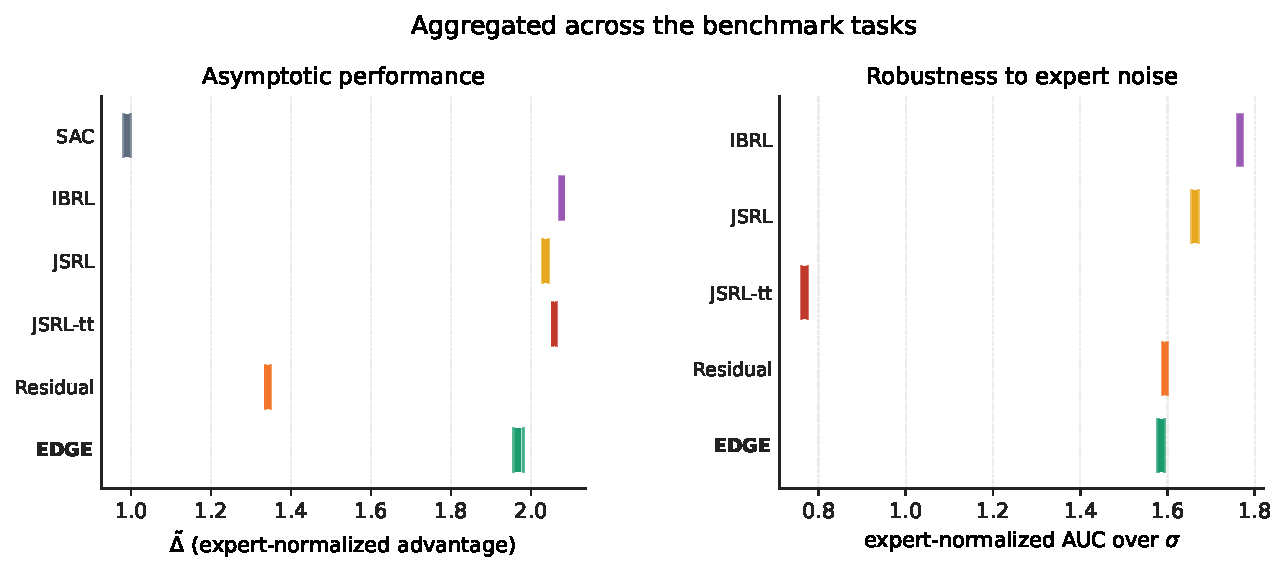
\includegraphics[width=0.92\linewidth]{figs/aggregated_rliable.pdf}
\caption{Aggregated results. Per-method IQM (vertical tick) with the
inter-quartile range of the stratified bootstrap shown as a
horizontal rectangle (Q1 to Q3). Two scalar axes: asymptotic
$\nbias$ (left) and robustness to expert noise (right; mean
$\nbias$ over the $\sigma$ sweep). Sample-efficiency curves are in
Appendix~\ref{app:perenv}.}
\label{fig:aggregated}
\end{figure}

Table~\ref{tab:main_perenv} reports per-env asymptotic $\nbias$
(breakdown of Figure~\ref{fig:aggregated} leftmost panel).

\begin{table}[h]
\centering
\small
\renewcommand{\arraystretch}{1.3}
\begin{tabular}{lrrrrrr}
\toprule
\textbf{Method} & \textbf{P3D-Circle} & \textbf{P3D-Fig8} & \textbf{FourTank}
 & \textbf{GlassFurnace} & \textbf{CheetahRun} & \textbf{Barkour} \\
\midrule
Expert only              &  0.00 & 0.00 & 0.00 & 0.00 & 0.00 & 0.00 \\
SAC (baseline)           & -2.08 & TBD  & -0.04 & TBD & 0.44  & TBD \\
IBRL                     &  0.91 & TBD  & -0.06 & TBD & TBD   & TBD \\
JSRL (curriculum)        &  0.86 & TBD  & -0.06 & TBD & TBD   & TBD \\
JSRL (training-time)     &  0.93 & TBD  & -0.07 & TBD & TBD   & TBD \\
Residual SAC             & -0.48 & TBD  & -0.01 & TBD & TBD   & TBD \\
\midrule
\textbf{EDGE (ours)}     &  0.89 & TBD  & -0.04 & TBD & 0.50  & TBD \\
\bottomrule
\end{tabular}
\caption{Per-env asymptotic $\nbias$ (Eq.~\ref{eq:nbias}). IQM across
the per-task seed count. TBD cells pending; per-env curves and
degradation in Appendix~\ref{app:perenv}.}
\label{tab:main_perenv}
\end{table}

\subsection{Robustness to Expert Sub-Optimality}
\label{sec:sensitivity}

We perturb expert actions as
$a_{\mathrm{deg}} = \mathrm{clip}(a^\star + \sigma\mathcal{N}(0,I),
-1, 1)$ for $\sigma \in \{0.25, 0.5, 0.75\}$ and report end-of-training
$\Delta = J - J_{\mathrm{exp}}$ against the original (unperturbed)
expert. This isolates one failure mode of an imperfect expert
(zero-mean per-step jitter) and does not cover others a deployed
controller may exhibit (constant bias, latency, partial state
observability, distribution shift between calibration and deployment
regimes). We frame the result as a stress test for action-noise
robustness, not a complete robustness picture, and read EDGE's
worst-case behaviour on this axis as evidence for one form of
robustness rather than for robustness in general. The cross-task
aggregate is the right panel of Figure~\ref{fig:aggregated};
per-task curves and bar views are in Appendix~\ref{app:perenv}.
Ablations of EDGE's four design choices are in
Appendix~\ref{app:ablation}.

% ============================================================
\section{Discussion}
\label{sec:discussion}
% ============================================================

\subsection{Why Quality-Aware Mixing Works}

The state-dependent stochastic gate produces a replay buffer that
mixes expert and policy transitions at every visited state, so the
critic receives Bellman anchors at both action distributions; argmax
produces a near-deterministic buffer that anchors only the expert
arm, leaving the SAC actor to climb a miscalibrated $Q$-surface at
exactly the states where the expert dominates (extended discussion
in Appendix~\ref{app:proofs}).

\subsection{A Taxonomy of Expert-Guided RL Failure Modes}
\label{sec:failuremodes}

The benchmark exposes three mechanism-specific failure modes of
expert-guided RL, each tied to a structural property of the expert
or the integration mechanism. Naming them lets us predict, rather
than merely report, which method fails on which task.

\paragraph{F1: Critic blind spot (argmax-gating methods).}
\emph{Mechanism.} IBRL's argmax action selection plus IBRL bootstrap
stores expert transitions whenever the expert wins in $Q$, so the
critic receives no Bellman targets at the policy's own actions on
the expert-dominant set. The SAC actor reads
$Q_\phi(s, \pi_\theta(s))$ and optimizes against an unanchored
$Q$-surface. \emph{Diagnostic.} On near-ceiling-expert tasks the
expert dominates persistently, the blind spot grows, and IBRL ends
up \emph{below} pure SAC. The pre-registered one-sided permutation
test on FourTank confirms the directional prediction
(\S\ref{sec:protocol}, $p = 0.034$, $50$ seeds). \emph{Predicted
cells of failure.} Any task where the expert sits within $\sim 10\%$
of the achievable ceiling: in our suite, FourTank and GlassFurnace.
\emph{Falsification target on held-out task.} Plane3DFigureEight has
an expert at $\sim 3\%$ of optimum (well below the ceiling
threshold), so F1 predicts that IBRL is \emph{not} dominated by
no-expert SAC on this task. If the held-out evaluation finds IBRL
below pure SAC on Plane3DFigureEight despite the weak expert, the
F1 mechanism is wrong and the taxonomy needs revision.
\emph{Defence.} Stochastic gating with non-zero policy-action
sampling rate, which is what EDGE's softmax form provides; the
formal coverage statement is in Appendix~\ref{app:proofs}.

\paragraph{F2: Residual saturation (additive-correction methods).}
\emph{Mechanism.} Residual SAC executes $a = \mathrm{clip}(a^* + \Delta,
-1, 1)$ with $\Delta$ a learned correction in $[-1, 1]$. When the
expert is far from the optimal policy, the required correction
exceeds the residual's bounded scale and the method cannot recover,
regardless of training budget. \emph{Diagnostic.} Residual SAC's
clean-task gap to the per-env best correlates inversely with expert
quality: $0\%$ on FourTank (PID at $92\%$ of MPC oracle), $9\%$ on
CheetahRun (CPG at $\sim 36\%$ of RL ceiling), $64\%$ on
Plane3DCircle (PID at $\sim 53\%$ of MPC oracle). \emph{Predicted
cells of failure.} Tasks where the expert covers a region of the
action space far from the optimal policy's: in our suite,
Plane3DCircle, Plane3DFigureEight, and BarkourJoystick (the trot
expert cannot strafe or yaw). \emph{Defence.} Mixing-form methods
(IBRL, JSRL, EDGE) execute the policy action directly when chosen
and have no scale bound on the correction.

\paragraph{F3: Warm-start buffer poisoning (training-time handoff).}
\emph{Mechanism.} The training-time JSRL variant runs the expert for
the first $\rho T$ steps, then hands off to the policy. The replay
buffer accumulated during the warm-start phase reflects the expert's
state distribution, including any noise; after handoff, the policy
trains on the poisoned buffer with no recovery channel and no
ongoing expert demonstrations to anchor it. \emph{Diagnostic.} On
clean experts JSRL-training-time achieves the strongest mean
asymptote across the suite; under expert action-noise
($\sigma = 0.25$, $0.5$, $0.75$) it loses $79\%$ of clean return on
CheetahRun ($774 \to 161$ at $\sigma = 0.5$), $17\%$ on FourTank
($238 \to 196$), and reverses sign on Plane3DCircle ($+9488 \to
-8276$) -- the largest sensitivity to expert noise of any method we
evaluate. \emph{Predicted
cells of failure.} Any deployment where the expert's per-step
behaviour during training is itself noisy, mistuned, or drifts
relative to evaluation; the standard clean-expert protocol does not
surface this. \emph{Defence.} Curriculum-style or per-step
mixing methods (JSRL-curriculum, EDGE) keep the expert online
throughout training and can re-anchor when expert behaviour
degrades.

\paragraph{Reading the cells through the taxonomy.}
Each cell of degradation failure in
Figure~\ref{fig:aggregated} corresponds to one of F1--F3, not to
generic ``method X is worse here.'' The asymptote-strongest method
under clean evaluation (JSRL-training-time) and the
degradation-strongest method (EDGE / JSRL-curriculum, tied) are
governed by different mechanisms; this is the methodological reason
the standard clean-expert protocol can recommend a method that is
brittle by construction.

\paragraph{What this implies for the field.}
The standard expert-guided RL evaluation reports a single asymptote
per method per task. Two of the three failure modes above (F1 and
F3) are invisible under that protocol: F1 produces a method that
looks fine on clean evaluation but is silently dominated by no-expert
SAC on near-ceiling-expert tasks; F3 produces a method that looks
\emph{best} on clean evaluation but collapses under any expert
imperfection. F2 is the only mode the standard protocol catches.
We treat this as a methodological finding about the field, not a
finding about any individual method.

\paragraph{Some near-MPC-tuned experts cannot be surpassed at
$1\mathrm{M}$ steps.}
Orthogonal to the failure-mode taxonomy: on FourTank and
(preliminarily) GlassFurnace, no method exceeds the expert's mean
return. The PIDs are near the analytic ceiling (FourTank: within
$7\%$ of the MPC oracle), leaving little discoverable headroom. The
practitioner question becomes which method's ordering reveals useful
structure (\S\ref{sec:when-to-use}). We treat this as a calibration
of expectation, against the field-wide tendency to overclaim.

\subsection{Tuned Pessimism and Gate Sharpness Vary by Task}
\label{sec:beta-finding}

HPO settles on dramatically different positions on the
optimism-pessimism axis (parameterized by $\beta$) and the gate
sharpness axis (parameterized by $\tau$, see
\S\ref{sec:bandit}) depending on task structure
(Table~\ref{tab:beta_per_task}). The 30$\times$ spread of tuned
$\beta$ across envs (0.12 to 4.05) and the 50$\times$ spread of
$\tau$ (0.17 to 8.51) demonstrate that both axes are load-bearing
and exploitable: HPO finds different gate calibrations for
different task structures, not arbitrary noise. The mapping is
multidimensional and not fully resolved here, but a partial reading
is visible: P3DCircle (catastrophic failure, weak expert) lands at
strong pessimism with a wide gate ($\beta = 4.05$, $\tau = 8.51$,
i.e.\ very soft mixing); CheetahRun (no termination, weak expert)
lands at moderate pessimism with a near-deterministic gate;
FourTank (no termination, near-ceiling expert) lands at the lower
bound of $\beta$ with a moderate $\tau$.

\paragraph{Boundary signal on FourTank: extended-range follow-up.}
Standard HPO bounds $\beta \in [0.1, 5.0]$ log-scale and
$\tau \in [0.1, 10.0]$ log-scale, so neither the optimistic regime
($\beta < 0$) nor the IBRL limit ($\tau \to 0$) is reachable.
FourTank's saturation at $\beta = 0.12$ motivated an extended-range
variant (\textbf{edge-qa-opt}, restricted to FourTank,
$\beta \in \pm[0.1, 5.0]$ via signed-log, $\tau \in [0.001, 10.0]$
log-scale; see \S\ref{sec:bandit}) which is currently mid-phase1
($17/30$ trials). Preliminary results contradict the
``saturated-bound implies hidden optimistic optimum'' hypothesis:
HPO has sampled negative $\beta$ in $\sim$1/3 of trials (range
$-3.9$ to $+3.2$), but the top-4 phase1 trials are all positive
$\beta \in [0.16, 1.74]$ paired with very small $\tau \in [0.005,
0.01]$. The FourTank optimum appears to lie in the
\emph{near-IBRL} corner of the $(\beta, \tau)$ surface (small positive
$\beta$, $\tau \to 0$): enough stochasticity to avoid the
blind-spot of \S\ref{sec:method}, but a near-deterministic gate. The
binding HPO constraint on FourTank was the $\tau$ floor at $0.1$,
not the $\beta$ floor. Phase2 (top-5 at full budget) is pending and
will firm up the magnitudes; we report this as preliminary.

\begin{table}[h]
\centering
\small
\begin{tabular}{lcccc}
\toprule
\textbf{Task} & \textbf{Tuned $\beta$} & \textbf{Tuned $\tau$} & \textbf{Termination?} & \textbf{Expert quality} \\
\midrule
Plane3DCircle    & 4.05 & 8.51 & yes (crash) & weak (53\% of MPC) \\
GlassFurnace     & 3.61 & 0.28 & no          & moderate (75\%) \\
CheetahRun       & 1.16 & 0.17 & no          & weak (36\% of RL ceiling) \\
FourTank         & 0.12 (lower bound) & 1.64 & no & near-ceiling (92\% of MPC) \\
\midrule
\multicolumn{5}{l}{\emph{FourTank, extended-range HPO (edge-qa-opt; phase1, preliminary):}} \\
FourTank (top-1, p1) & $+0.35$ & $0.008$ & no & near-ceiling \\
FourTank (top-4 range, p1) & $+0.16$ to $+1.74$ & $0.002$ to $0.009$ & no & near-ceiling \\
\bottomrule
\end{tabular}
\caption{HPO-tuned $(\beta, \tau)$ for EDGE across four envs (phase3
complete) plus the extended-range follow-up on FourTank
(\S\ref{sec:bandit}; phase1, preliminary). The FourTank top-4
phase1 trials concentrate at small positive $\beta$ and very small
$\tau$, suggesting the binding constraint in the standard sweep was
the $\tau$ floor at $0.1$, not the $\beta$ floor.}
\label{tab:beta_per_task}
\end{table}

\subsection{Decision Rule: Which Method to Deploy When}
\label{sec:when-to-use}

The taxonomy of \S\ref{sec:failuremodes} converts the per-cell
results into a decision rule keyed on three observables a
practitioner can measure before training: expert quality $q$
(fraction of achievable return the expert attains), task termination
(catastrophic failure during exploration), and whether the expert is
expected to be perturbed at deploy time relative to its calibration.
Each branch of the rule is the unique method that avoids all three
failure modes F1--F3 on its branch.

\begin{enumerate}
\item \textbf{Expert quality $q \gtrsim 0.9$ on a non-terminating
task with smooth corrections.} F1 (critic blind spot) dominates the
risk; F2 (residual saturation) does not bind because the required
correction is small. \emph{Use Residual SAC.} Empirical anchor:
FourTank, where Residual is the only method to match the expert
($0\%$ clean gap) and IBRL is dominated by no-expert SAC
(pre-registered, $p = 0.034$).

\item \textbf{Expert quality $q \lesssim 0.6$ on a non-terminating
task.} F2 binds (residual saturation), so additive correction is
ruled out; F1 does not bind because the policy's Q quickly becomes
competitive. \emph{Use IBRL or JSRL-curriculum.} Empirical anchor:
CheetahRun, where IBRL and JSRL-curriculum lead and Residual trails
by $9\%$.

\item \textbf{Terminating task (catastrophic failure during
exploration).} F2 still binds whenever the expert is mid-quality,
and F1 binds whenever the expert ends up dominant; both rule out
Residual and IBRL. \emph{Use JSRL-curriculum or EDGE.} Empirical
anchor: Plane3DCircle, where Residual is at $-64\%$ and EDGE,
JSRL-curriculum, JSRL-tt, IBRL all cluster within $13\%$ of the
best.

\item \textbf{Expert expected to be perturbed at deployment relative
to its calibration regime.} F3 binds (warm-start poisoning), ruling
out the training-time JSRL variant. \emph{Use JSRL-curriculum or
EDGE.} Empirical anchor: degradation cells, where JSRL-tt's worst
gap is $> 200\%$ and JSRL-curriculum / EDGE are tied at $13\%$.

\item \textbf{Joint conditions (catastrophic failure \emph{and}
expected expert perturbation).} JSRL-curriculum and EDGE remain;
they are statistically tied on aggregate. \emph{Use either; we
recommend EDGE when the expert's quality varies across the state
space, since EDGE's gate is state-conditional and JSRL-curriculum's
horizon schedule is not.}
\end{enumerate}

The rule is fitted to the cells we have. We hold out
Plane3DFigureEight (a stress variant of Plane3DCircle with a
near-broken expert) for validation; the rule predicts
JSRL-curriculum or EDGE on the catastrophic-failure branch, and the
empirical results in Appendix~\ref{app:perenv} test this prediction.
The single-condition branches each have only one or two empirical
anchors, so the rule should be read as predictive guidance to
falsify rather than a closed result; the next deadline iteration
extends the empirical base to more cells.

\subsection{Limitations}

EDGE requires a queryable expert at every visited state (fixed-dataset
demonstrations do not satisfy this), assumes dense rewards, and
requires an ensemble critic with non-degenerate disagreement (single
critics degrade the gate to a deterministic margin comparison). Scope
extensions and per-step compute are in
Appendix~\ref{app:limitations_extra}.

% ============================================================
\section{Conclusion}
\label{sec:conclusion}
% ============================================================

Our benchmark of five expert-guided RL methods reveals that
JSRL-training-time, the asymptote-strongest baseline, is the most
degradation-fragile; that Residual SAC dominates the
near-optimal-expert smooth-control niche where IBRL's argmax
bootstrap is harmful via the blind spot of \S\ref{sec:method}; and
that EDGE, our quality-aware ensemble-pessimism-gated method, is
competitive everywhere and uniquely robust under expert
action-noise. EDGE is the recommended default whenever expert
quality at deploy is uncertain.

\paragraph{Future work: literal pessimistic Thompson sampling.}
A literal pessimistic-TS instantiation (per-arm ensemble draw,
argmax over LCB-shifted samples) would carry a Bayesian regret
bound \citep{russo2014ts} and remove $\tau$ as a hyperparameter.
This requires a critic ensemble large enough for the posterior to
actually disperse: published results
\citep{an2021edac,ghasemipour2022msg} suggest $K \geq 10$ with an
explicit diversification loss. Our HPO uses $K \in \{2, 4\}$, well
below that regime, so the Gaussian approximation EDGE uses (with
$\tau$ compensating for under-dispersion) is the defensible choice
at our compute budget. Scaling the ensemble and benchmarking
literal pessimistic TS against the EDGE Gaussian approximation is a
natural follow-up; we predict the two will converge at sufficient
$K$ and that $\tau$ becomes redundant in that limit.




% ============================================================
\bibliographystyle{plainnat}
\begin{thebibliography}{99}

\bibitem[Agarwal et al.(2021)]{agarwal2021rliable}
R.~Agarwal, M.~Schwarzer, P.~S. Castro, A.~C. Courville, and M.~G. Bellemare.
\newblock Deep reinforcement learning at the edge of the statistical precipice.
\newblock In \emph{NeurIPS}, 2021.
\newblock URL \url{https://proceedings.neurips.cc/paper/2021/hash/f514cec81cb148559cf475e7426eed5e-Abstract.html}.

\bibitem[Ball et al.(2023)]{ball2023rlpd}
P.~Ball, L.~Smith, I.~Kostrikov, and S.~Levine.
\newblock Efficient online reinforcement learning with offline data.
\newblock In \emph{ICML}, 2023.
\newblock URL \url{https://proceedings.mlr.press/v202/ball23a.html}.

\bibitem[Haarnoja et al.(2018)]{haarnoja2018sac}
T.~Haarnoja, A.~Zhou, P.~Abbeel, and S.~Levine.
\newblock Soft actor-critic: Off-policy maximum entropy deep reinforcement
    learning with a stochastic actor.
\newblock In \emph{ICML}, 2018.
\newblock URL \url{https://proceedings.mlr.press/v80/haarnoja18b.html}.

\bibitem[Hu et al.(2024)]{hu2023ibrl}
H.~Hu, S.~Mirchandani, and D.~Sadigh.
\newblock Imitation bootstrapped reinforcement learning.
\newblock In \emph{RSS}, 2024.
\newblock URL \url{https://www.roboticsproceedings.org/rss20/p089.html}.

\bibitem[Johannink et al.(2019)]{johannink2019residual}
T.~Johannink, S.~Bahl, A.~Nair, J.~Luo, A.~Kumar, M.~Loskyll,
    J.~A. Ojea, E.~Solowjow, and S.~Levine.
\newblock Residual reinforcement learning for robot control.
\newblock In \emph{ICRA}, 2019.
\newblock URL \url{https://ieeexplore.ieee.org/document/8794127}.

\bibitem[Lee et al.(2021)]{lee2021sunrise}
K.~Lee, M.~Laskin, A.~Srinivas, and P.~Abbeel.
\newblock {SUNRISE}: A simple unified framework for ensemble learning in deep RL.
\newblock In \emph{ICML}, 2021.
\newblock URL \url{https://proceedings.mlr.press/v139/lee21g.html}.

\bibitem[Nair et al.(2020)]{nair2020awac}
A.~Nair, M.~Dalal, A.~Gupta, and S.~Levine.
\newblock {AWAC}: Accelerating online reinforcement learning with offline datasets.
\newblock \emph{arXiv:2006.09359}, 2020.
\newblock URL \url{https://arxiv.org/abs/2006.09359}.

\bibitem[Ross et al.(2011)]{ross2011dagger}
S.~Ross, G.~Gordon, and D.~Bagnell.
\newblock A reduction of imitation learning and structured prediction to
    no-regret online learning.
\newblock In \emph{AISTATS}, 2011.
\newblock URL \url{https://proceedings.mlr.press/v15/ross11a.html}.

\bibitem[\r{A}str\"{o}m and H\"{a}gglund(1984)]{astrom1984relay}
K.~J. \r{A}str\"{o}m and T.~H\"{a}gglund.
\newblock Automatic tuning of simple regulators with specifications on phase
    and amplitude margins.
\newblock \emph{Automatica}, 20(5):645--651, 1984.
\newblock URL \url{https://doi.org/10.1016/0005-1098(84)90014-1}.

\bibitem[\r{A}str\"{o}m and H\"{a}gglund(2005)]{astrom2005amigo}
K.~J. \r{A}str\"{o}m and T.~H\"{a}gglund.
\newblock \emph{Advanced PID Control}.
\newblock ISA, 2005.
\newblock URL \url{https://www.isa.org/products/advanced-pid-control}.

\bibitem[Ijspeert(2008)]{ijspeert2008cpg}
A.~J. Ijspeert.
\newblock Central pattern generators for locomotion control in animals and
    robots: a review.
\newblock \emph{Neural Networks}, 21(4):642--653, 2008.
\newblock URL \url{https://doi.org/10.1016/j.neunet.2008.03.014}.

\bibitem[Russo and Van Roy(2014)]{russo2014ts}
D.~Russo and B.~Van~Roy.
\newblock Learning to optimize via posterior sampling.
\newblock \emph{Mathematics of Operations Research}, 39(4):1221--1243, 2014.
\newblock URL \url{https://doi.org/10.1287/moor.2014.0650}.

\bibitem[Russo et al.(2018)]{russo2018tutorial}
D.~Russo, B.~Van~Roy, A.~Kazerouni, I.~Osband, and Z.~Wen.
\newblock A tutorial on Thompson sampling.
\newblock \emph{Foundations and Trends in Machine Learning}, 11(1):1--96, 2018.
\newblock URL \url{https://doi.org/10.1561/2200000070}.

\bibitem[Osband et al.(2016)]{osband2016bootstrappeddqn}
I.~Osband, C.~Blundell, A.~Pritzel, and B.~Van~Roy.
\newblock Deep exploration via bootstrapped DQN.
\newblock In \emph{NeurIPS}, 2016.
\newblock URL \url{https://proceedings.neurips.cc/paper/2016/hash/8d8818c8e140c64c743113f563cf750f-Abstract.html}.

\bibitem[An et al.(2021)]{an2021edac}
G.~An, S.~Moon, J.-H. Kim, and H.~O. Song.
\newblock Uncertainty-based offline reinforcement learning with diversified
    Q-ensemble.
\newblock In \emph{NeurIPS}, 2021.
\newblock URL \url{https://proceedings.neurips.cc/paper/2021/hash/3d3d286a8d153a4a58156d0e02d8570c-Abstract.html}.

\bibitem[Ghasemipour et al.(2022)]{ghasemipour2022msg}
S.~K.~S. Ghasemipour, S.~S. Gu, and O.~Nachum.
\newblock Why so pessimistic? Estimating uncertainties for offline RL through
    ensembles, and why their independence matters.
\newblock In \emph{NeurIPS}, 2022.
\newblock URL \url{https://proceedings.neurips.cc/paper_files/paper/2022/hash/7b1ca40a4c4326e4b95a3da8e7b81f73-Abstract-Conference.html}.

\bibitem[Lattimore and Szepesv\'{a}ri(2020)]{lattimore2020bandit}
T.~Lattimore and C.~Szepesv\'{a}ri.
\newblock \emph{Bandit Algorithms}.
\newblock Cambridge University Press, 2020.
\newblock URL \url{https://tor-lattimore.com/downloads/book/book.pdf}.

\bibitem[Wu et al.(2016)]{wu2016conservative}
Y.~Wu, R.~Shariff, T.~Lattimore, and C.~Szepesv\'{a}ri.
\newblock Conservative bandits.
\newblock In \emph{ICML}, 2016.
\newblock URL \url{https://proceedings.mlr.press/v48/wu16.html}.

\bibitem[Kazerouni et al.(2017)]{kazerouni2017conservative}
A.~Kazerouni, M.~Ghavamzadeh, Y.~Abbasi-Yadkori, and B.~Van~Roy.
\newblock Conservative contextual linear bandits.
\newblock In \emph{NeurIPS}, 2017.
\newblock URL \url{https://proceedings.neurips.cc/paper/2017/hash/bdc4626aa1d1df8e14d80d345b2a442d-Abstract.html}.

\bibitem[Abe and Long(1999)]{abe1999igw}
N.~Abe and P.~M. Long.
\newblock Associative reinforcement learning using linear probabilistic
    concepts.
\newblock In \emph{ICML}, 1999.
\newblock URL \url{https://www.aaai.org/Papers/ICML/1999/ICML99-002.pdf}.

\bibitem[Johansson(2000)]{johansson2000quadruple}
K.~H. Johansson.
\newblock The quadruple-tank process: A multivariable laboratory process with
    an adjustable zero.
\newblock \emph{IEEE Transactions on Control Systems Technology}, 8(3):456--465,
    2000.
\newblock URL \url{https://doi.org/10.1109/87.845876}.

\bibitem[Lewis(2008)]{lewis2008nuclear}
E.~E. Lewis.
\newblock \emph{Fundamentals of Nuclear Reactor Physics}.
\newblock Academic Press, 2008.
\newblock URL \url{https://www.elsevier.com/books/fundamentals-of-nuclear-reactor-physics/lewis/978-0-12-370631-7}.

\bibitem[Storn and Price(1997)]{storn1997de}
R.~Storn and K.~Price.
\newblock Differential evolution, a simple and efficient heuristic for global
    optimization over continuous spaces.
\newblock \emph{Journal of Global Optimization}, 11(4):341--359, 1997.
\newblock URL \url{https://doi.org/10.1023/A:1008202821328}.

\bibitem[Uchendu et al.(2023)]{uchendu2023jsrl}
I.~Uchendu, T.~Xiao, Y.~Lu, B.~Zhu, M.~Yan, J.~Simon, M.~Bennice,
    C.~Fu, C.~Ma, J.~Jiao, S.~Levine, and K.~Hausman.
\newblock {JSRL}: Jump-start reinforcement learning.
\newblock In \emph{ICML}, 2023.
\newblock URL \url{https://proceedings.mlr.press/v202/uchendu23a.html}.

\bibitem[Zhang et al.(2023)]{zhang2023pex}
H.~Zhang, W.~Xu, and H.~Yu.
\newblock Policy expansion for bridging offline-to-online reinforcement
    learning.
\newblock In \emph{ICLR}, 2023.
\newblock URL \url{https://openreview.net/forum?id=-Y34L45JR6z}.

\bibitem[Rengarajan et al.(2022)]{rengarajan2022logo}
D.~Rengarajan, G.~Vaidya, A.~Sarvesh, D.~Kalathil, and S.~Shakkottai.
\newblock Reinforcement learning with sparse rewards using guidance from
    offline demonstration.
\newblock In \emph{ICLR}, 2022.
\newblock URL \url{https://openreview.net/forum?id=YJ1WzgMVsMt}.

\bibitem[Kostrikov et al.(2022)]{kostrikov2022iql}
I.~Kostrikov, A.~Nair, and S.~Levine.
\newblock Offline reinforcement learning with implicit Q-learning.
\newblock In \emph{ICLR}, 2022.
\newblock URL \url{https://openreview.net/forum?id=68n2s9ZJWF8}.

\bibitem[Zakka et al.(2025)]{mujocoplayground2024}
K.~Zakka et al.
\newblock {MuJoCo Playground}: An open-source framework for GPU-accelerated
    robot learning and sim-to-real transfer.
\newblock \emph{arXiv:2502.08844}, 2025.
\newblock URL \url{https://arxiv.org/abs/2502.08844}.

\end{thebibliography}

% ============================================================
\appendix

\section{Critic Blind Spots: Extended Discussion and Proof}
\label{app:proofs}
% ============================================================

We state and prove the two formal results behind the informal
``critic blind spot'' motivation in Section~\ref{sec:method}.

\begin{remark}[Critic blind spot under argmax selection]
\label{rem:blindspot}
Let $\mathcal{M}_t = \{s : Q_\phi(s,\pi^*(s)) > \mathbb{E}_{a\sim
\pi_\theta(\cdot|s)} Q_\phi(s,a)\}$. Under IBRL-style argmax, no
fresh transition $(s, a, \cdot, \cdot)$ with $s\in\mathcal{M}_t$ and
$a\neq\pi^*(s)$ enters the buffer at step $t$. The Bellman regression
is therefore insensitive to $Q_\phi(s, \pi_\theta(s))$ on
$\mathcal{M}_t$ for as long as $\mathcal{M}_t$ persists.
\end{remark}

\begin{lemma}[Coverage under pessimism-gated mixing]
\label{lem:coverage}
Under the gate \eqref{eq:behavior} with finite pessimism gap, every
visited $s$ accumulates policy-action Bellman anchors at expected
rate $(1 - p_t(s))\,\mu_t(s) > 0$, so no persistent analogue of
$\mathcal{M}_t$ can form.
\end{lemma}

\paragraph{Why the bias is mechanistic.} Whenever the expert wins at
state $s$, IBRL-style argmax stores $(s, \pi^*(s), r, s')$ in the
replay buffer, and the critic's Bellman regression target on that
tuple anchors $Q_\phi(s, \pi^*(s))$, not $Q_\phi(s, a)$ for
$a \neq \pi^*(s)$. The SAC actor update reads
$\nabla_\theta \mathbb{E}_{s \sim \mathcal{B},\, a \sim \pi_\theta(\cdot
| s)}[Q_\phi(s, a) - \alpha \log \pi_\theta(a|s)]$: the stored action
does not enter the gradient directly, but the gradient's quality
depends on $Q_\phi(s, a)$ being calibrated for the actions
$\pi_\theta$ actually proposes. Older transitions written before
$\mathcal{M}_t$ took its current shape may anchor the policy arm,
but that anchor freezes as soon as the gap-sign flips:
$Q_\phi(s, \pi_\theta(s))$ on $\mathcal{M}_t$ is then determined by
stale data and function-approximator generalization, while it is
exactly the quantity the actor improves against. The failure is
mechanistic, not statistical: even with unlimited environment data,
pure argmax records no fresh transition whose Bellman target updates
$Q_\phi$ at policy-proposed actions on $\mathcal{M}_t$.

\begin{proof}[Proof of Lemma~\ref{lem:coverage}]
Conditional on the state, the gate is a Bernoulli draw with parameter
$p_t(s) = \sigma\big((\check{Q}_t(s,\pi^*(s)) - \check{Q}_t(s,
\pi_\theta(s)))/\tau\big)$. As the image of a finite real number
under the logistic, $p_t(s) \in (0, 1)$. The policy arm therefore
has positive mass at every visited $s$, and the per-step rate of
policy-action Bellman anchors at $s$ is exactly
$(1 - p_t(s))\,\mu_t(s)$ by the law of total probability over $\mu_t$.
\qedhere
\end{proof}


\section{Per-Environment Results}
\label{app:perenv}
% ============================================================

This appendix reports per-environment training curves, expert-bias
trajectories, and degradation curves underlying the aggregated
Figure~\ref{fig:aggregated} and Table~\ref{tab:main_perenv}. Aggregation
choices in the main text (expert-normalization, IQM across envs, stratified
bootstrap) are deliberate, but the per-env curves here are the raw evidence
behind them, so reviewers can verify nothing is hidden by aggregation.

\begin{figure}[h]
\centering
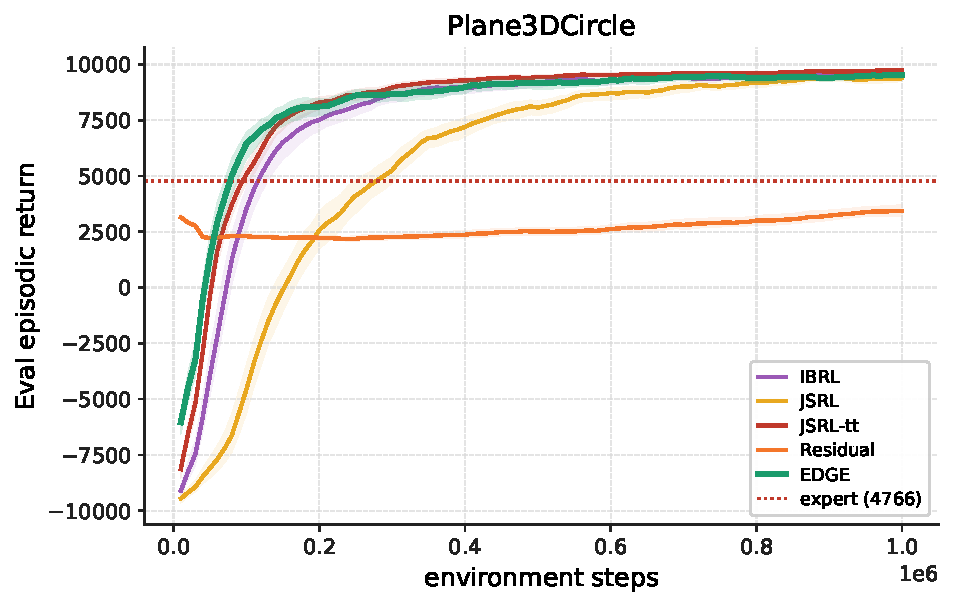
\includegraphics[width=0.48\linewidth]{figs/curves_plane3dcircle_Eval_episodic_mean_reward.pdf}\hfill
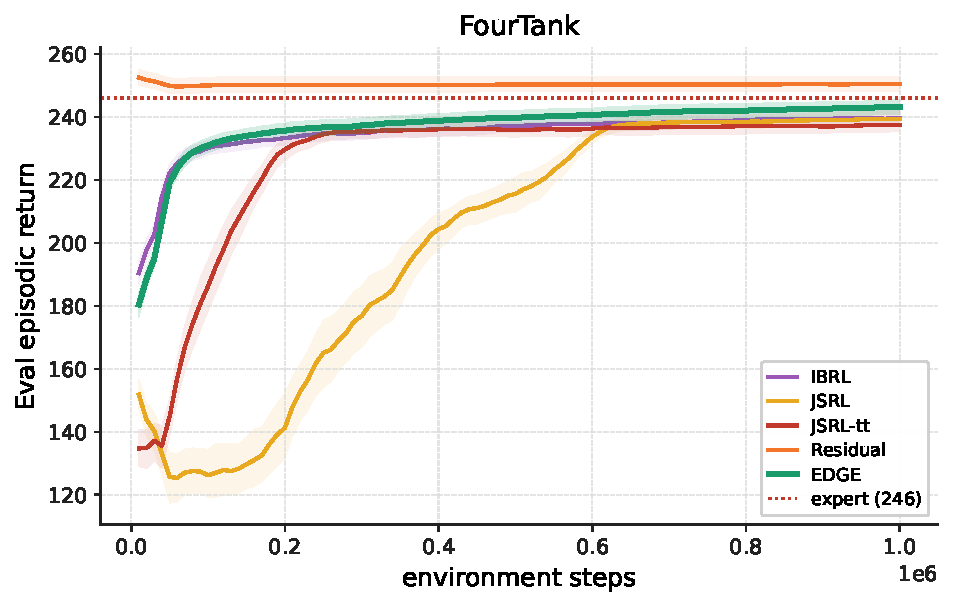
\includegraphics[width=0.48\linewidth]{figs/curves_fourtank_Eval_episodic_mean_reward.pdf}\\
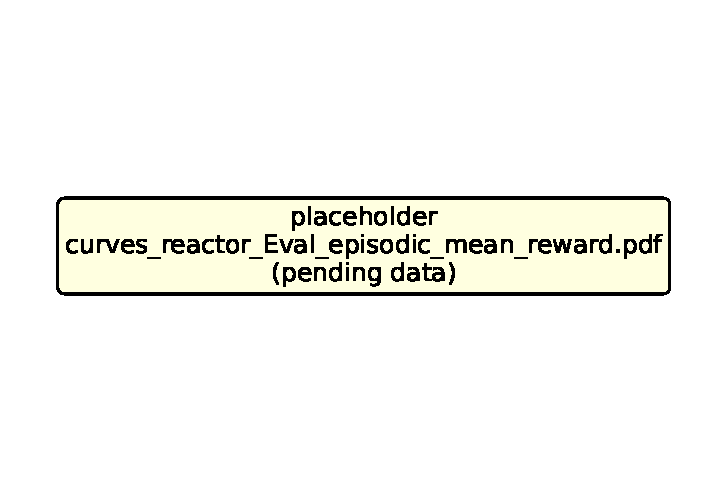
\includegraphics[width=0.48\linewidth]{figs/curves_reactor_Eval_episodic_mean_reward.pdf}\hfill
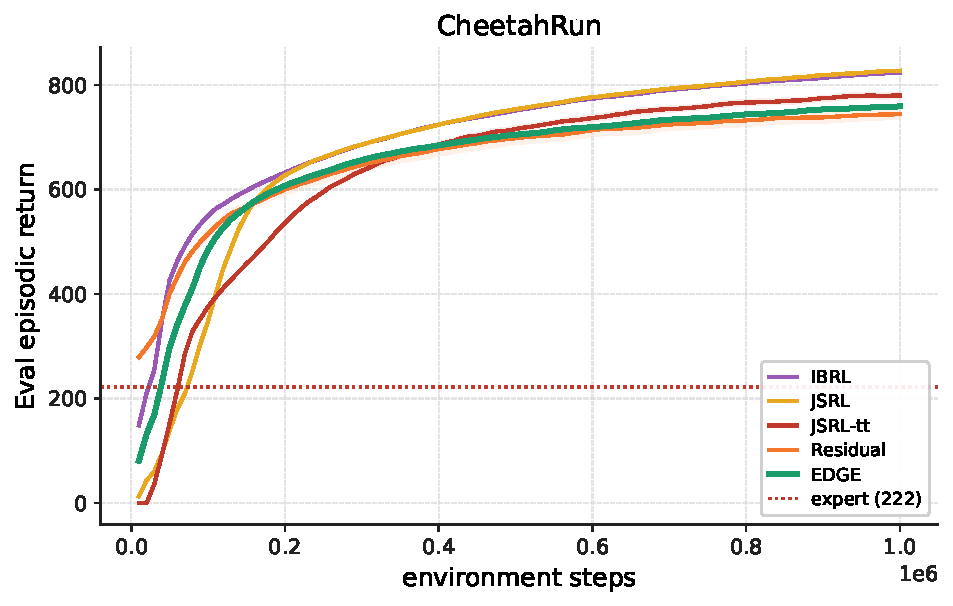
\includegraphics[width=0.48\linewidth]{figs/curves_cheetahrun_Eval_episodic_mean_reward.pdf}\\
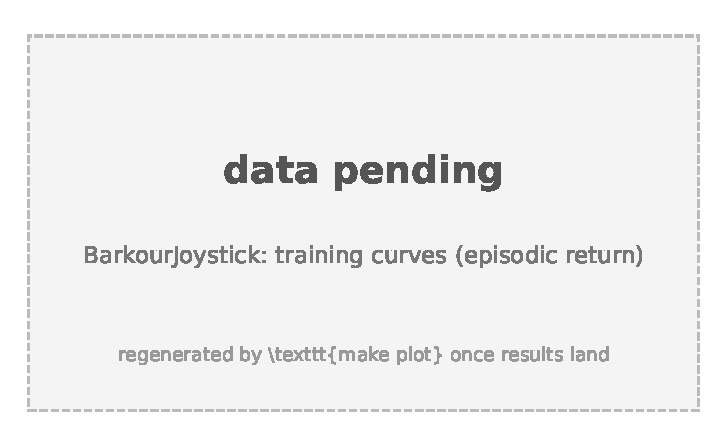
\includegraphics[width=0.48\linewidth]{figs/curves_barkourjoystick_Eval_episodic_mean_reward.pdf}
\caption{Per-environment learning curves. IQM across 100 seeds with
bootstrap 95\% CI band. Horizontal dashed line marks $J_{\text{exp}}$.
[Pending; figures regenerate from \texttt{plot\_sweep.py --paper}.]}
\label{fig:curves_appendix}
\end{figure}

\begin{figure}[h]
\centering
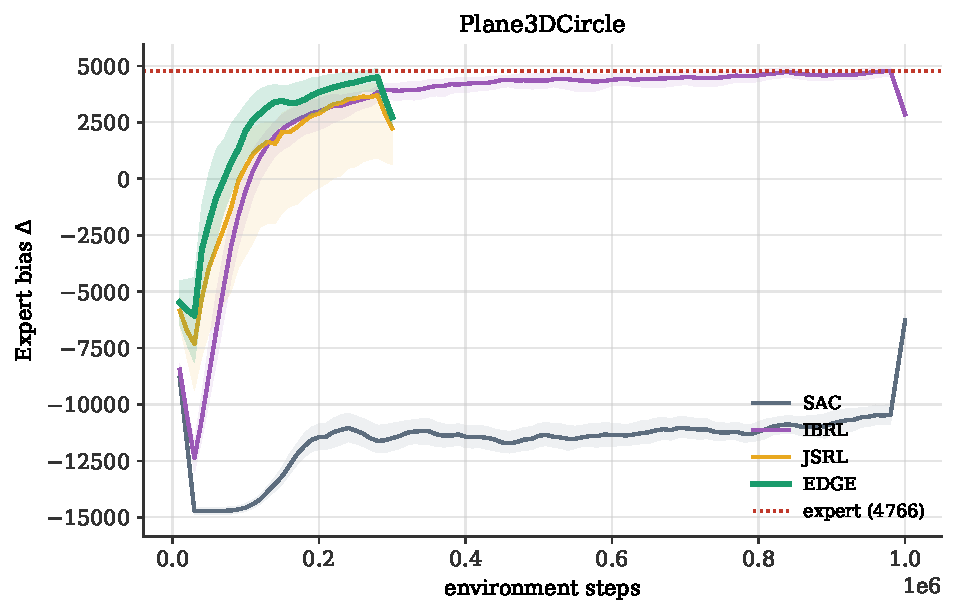
\includegraphics[width=0.48\linewidth]{figs/curves_plane3dcircle_Eval_expert_bias.pdf}\hfill
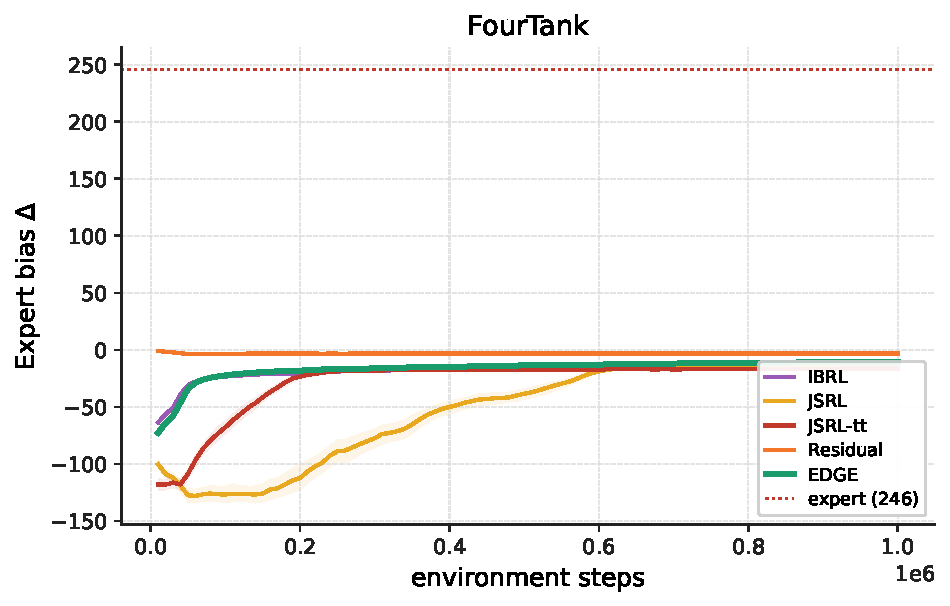
\includegraphics[width=0.48\linewidth]{figs/curves_fourtank_Eval_expert_bias.pdf}\\
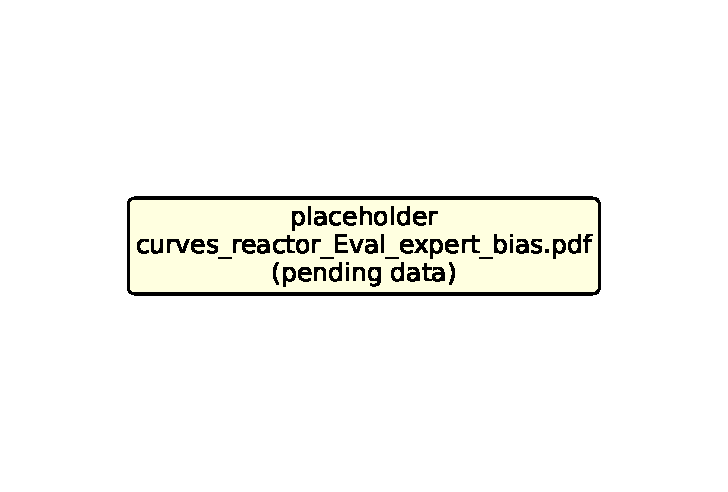
\includegraphics[width=0.48\linewidth]{figs/curves_reactor_Eval_expert_bias.pdf}\hfill
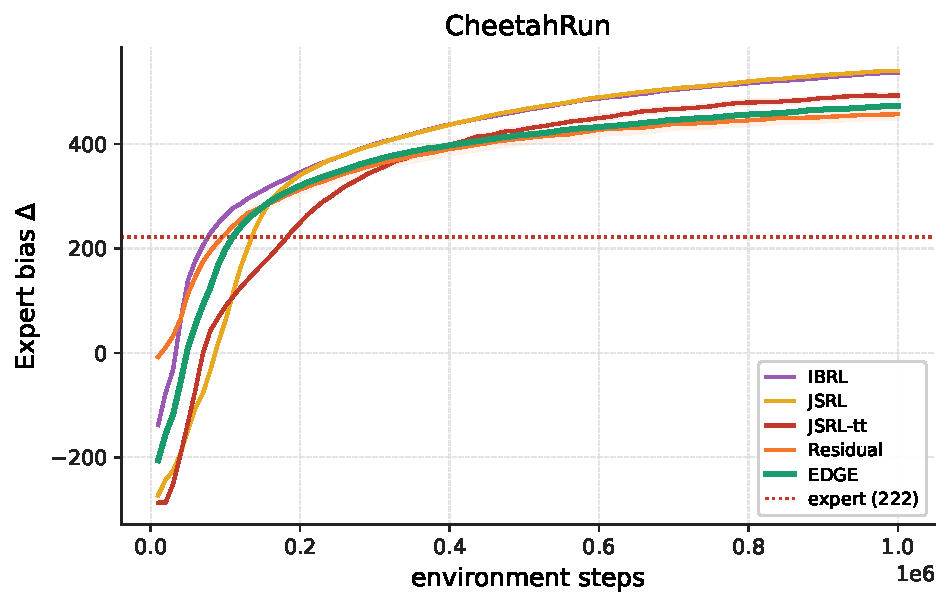
\includegraphics[width=0.48\linewidth]{figs/curves_cheetahrun_Eval_expert_bias.pdf}\\
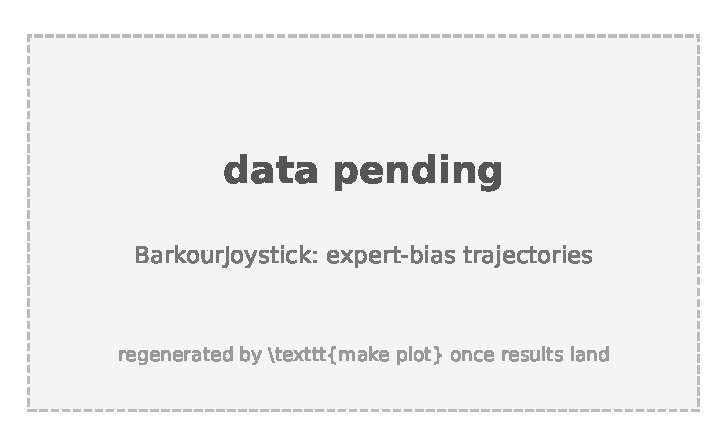
\includegraphics[width=0.48\linewidth]{figs/curves_barkourjoystick_Eval_expert_bias.pdf}
\caption{Per-environment expert bias $\Delta = J - J_{\text{exp}}$. The
horizontal axis at zero marks expert parity. [Pending.]}
\label{fig:bias_appendix}
\end{figure}

\begin{figure}[h]
\centering
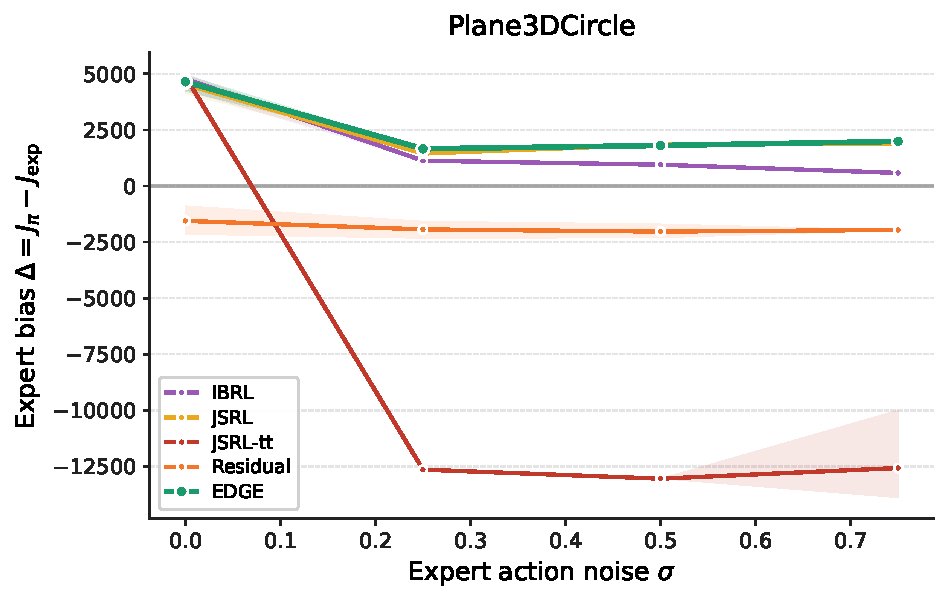
\includegraphics[width=0.48\linewidth]{figs/degradation_plane3dcircle.pdf}\hfill
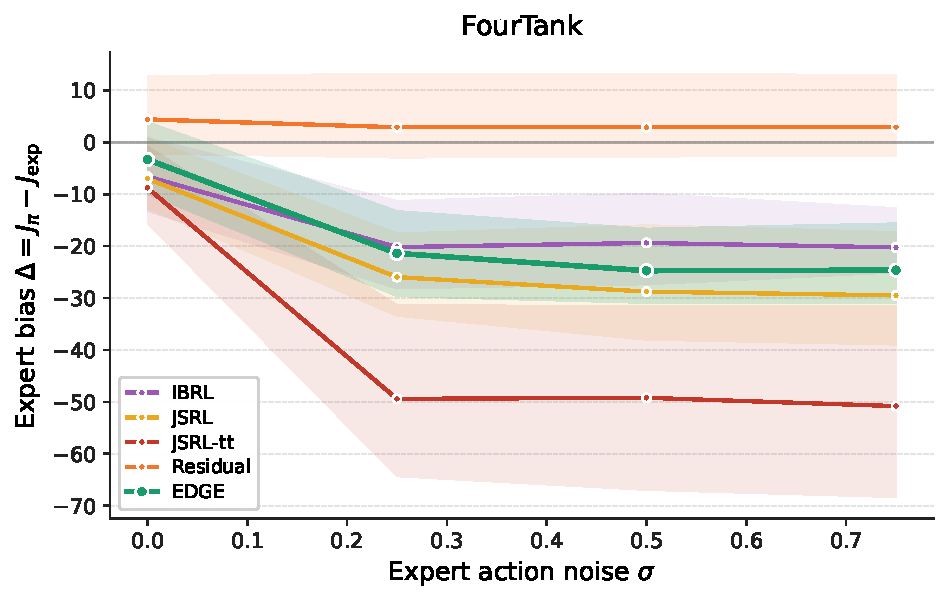
\includegraphics[width=0.48\linewidth]{figs/degradation_fourtank.pdf}\\
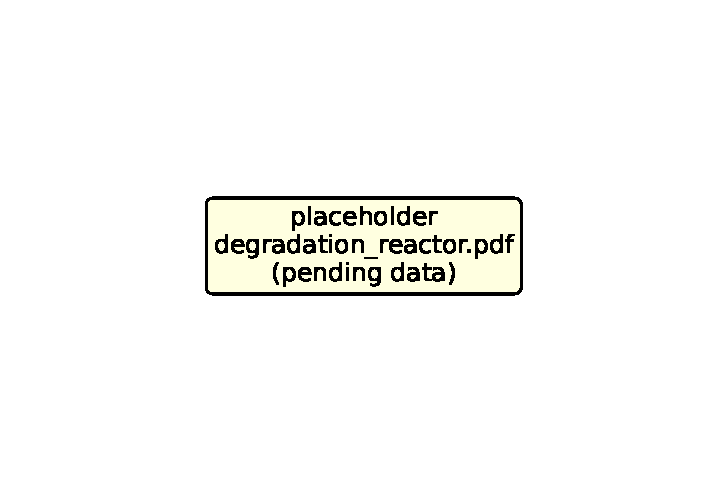
\includegraphics[width=0.48\linewidth]{figs/degradation_reactor.pdf}\hfill
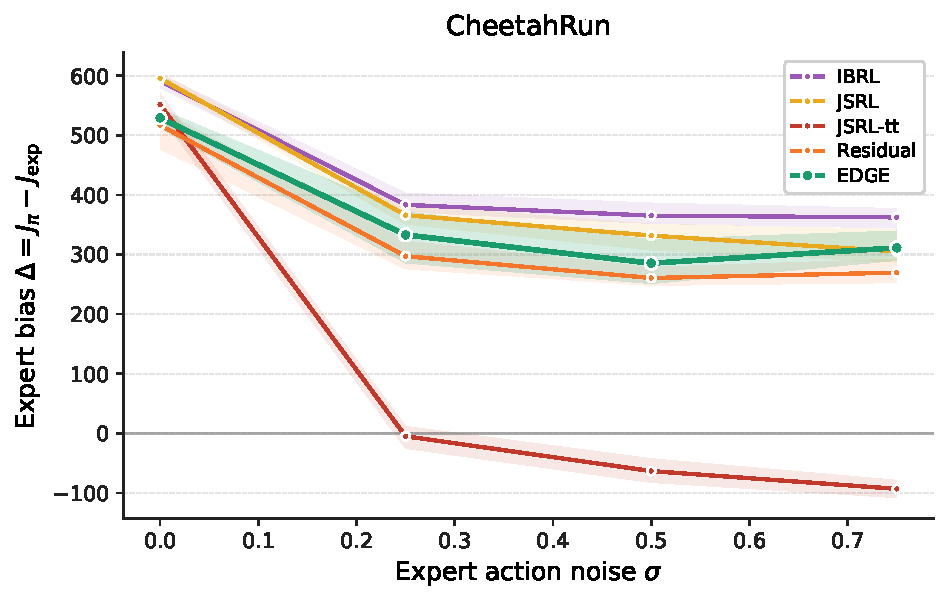
\includegraphics[width=0.48\linewidth]{figs/degradation_cheetahrun.pdf}\\
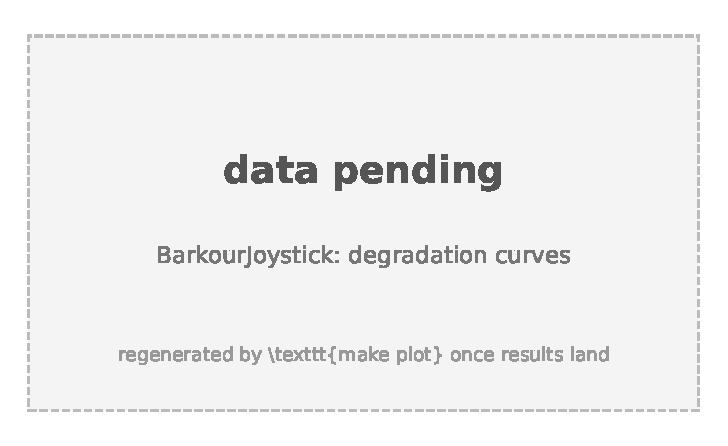
\includegraphics[width=0.48\linewidth]{figs/degradation_barkourjoystick.pdf}
\caption{Per-environment degradation: final eval reward as a function of
expert-action noise $\sigma$. Lower-bound at SAC reflects the expert-free
floor. [Pending.]}
\label{fig:degradation_appendix}
\end{figure}

\begin{figure}[h]
\centering
\IfFileExists{figs/degradation_bars_plane3dcircle.pdf}{%
  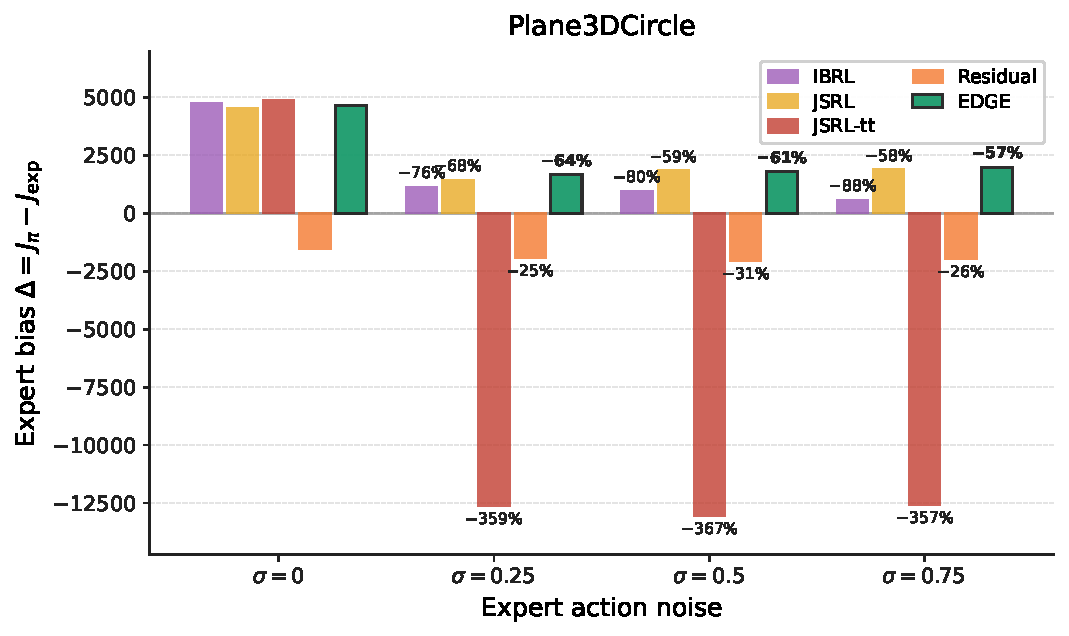
\includegraphics[width=0.48\linewidth]{figs/degradation_bars_plane3dcircle.pdf}}{}\hfill
\IfFileExists{figs/degradation_bars_fourtank.pdf}{%
  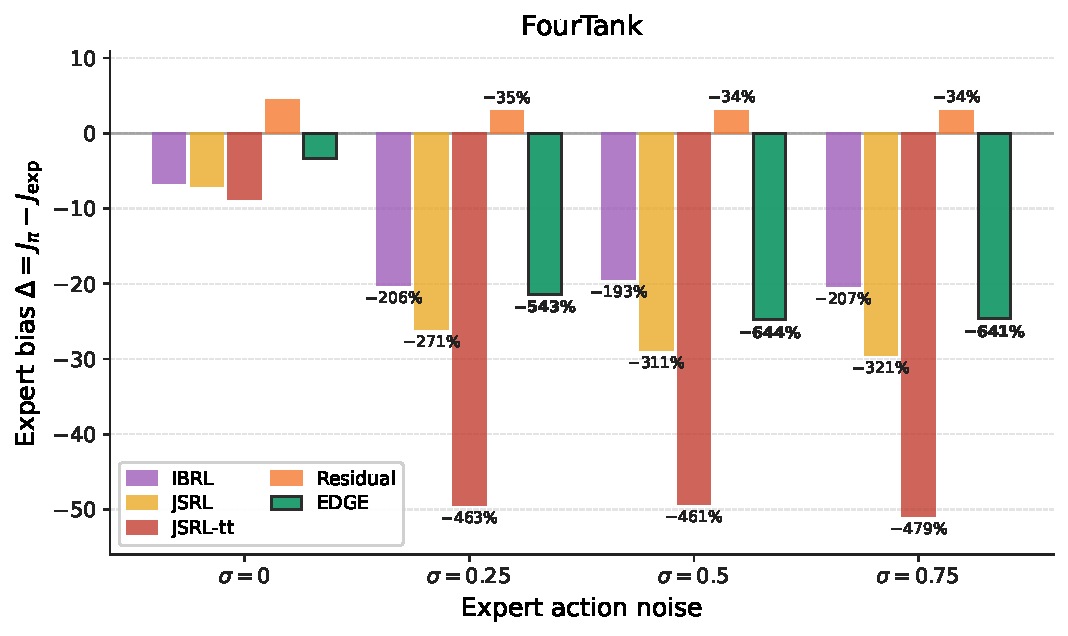
\includegraphics[width=0.48\linewidth]{figs/degradation_bars_fourtank.pdf}}{}\\
\IfFileExists{figs/degradation_bars_reactor.pdf}{%
  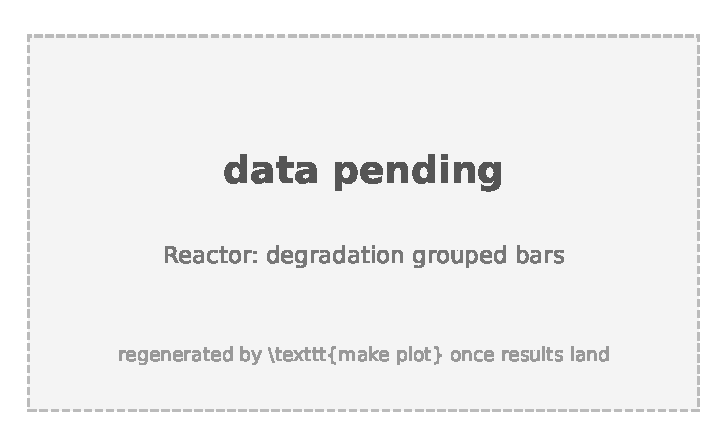
\includegraphics[width=0.48\linewidth]{figs/degradation_bars_reactor.pdf}}{}\hfill
\IfFileExists{figs/degradation_bars_cheetahrun.pdf}{%
  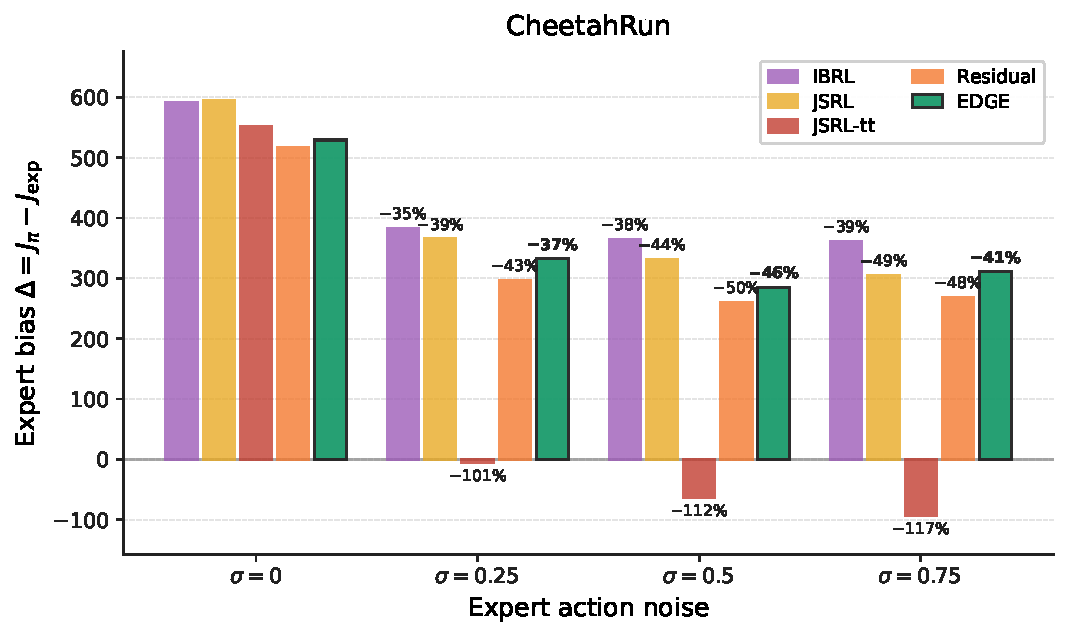
\includegraphics[width=0.48\linewidth]{figs/degradation_bars_cheetahrun.pdf}}{}\\
\IfFileExists{figs/degradation_bars_barkourjoystick.pdf}{%
  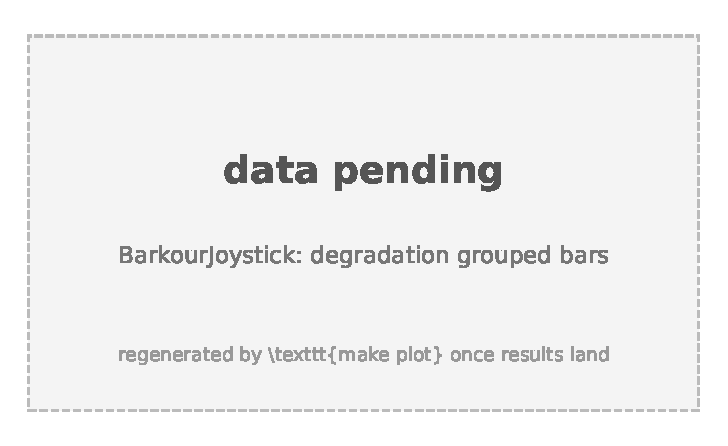
\includegraphics[width=0.48\linewidth]{figs/degradation_bars_barkourjoystick.pdf}}{}
\caption{Per-environment degradation, grouped-bar view. Each group of
bars corresponds to one expert-noise level $\sigma\in\{0, 0.25, 0.5,
0.75\}$; one bar per method. Easier to read than the line plot when
methods collapse to very different scales (e.g.\ residual SAC and
JSRL training-time on Plane3DCircle).}
\label{fig:degradation_bars_appendix}
\end{figure}

\section{Ablation Study}
\label{app:ablation}
% ============================================================

EDGE composes two design choices the abstract foregrounds (gating
form and pessimism) plus four secondary choices (preprocessing,
critic bootstrap, expert quality sanity, off-policy correctness).
Each variant below flips a single knob of the tuned EDGE-QA config
from the \texttt{sac\_quality\_aware} HPO study and retrains at the
same per-task seed count as the main study (50 seeds,
$1\mathrm{M}$ steps). Variants run on Plane3DCircle and CheetahRun:
Plane3DCircle has the largest between-method spread of any benchmark
task and gives clean signal-to-noise for design-choice ablations;
CheetahRun stresses the same knobs on a non-terminating task with a
weak expert. FourTank is excluded as an ablation env because the
per-seed standard deviation ($\sim 10$ on a $\sim 240$ scale) makes
sub-method-swap effects borderline even with $50$ seeds.

\paragraph{Variant $\to$ axis map.}
\begin{center}
\small
\begin{tabular}{lll}
\toprule
\textbf{Variant} & \textbf{Knob flipped} & \textbf{Axis tested} \\
\midrule
\texttt{gating\_argmax}        & softmax over LCB $\to$ argmax over mean-$Q$ & gating form $\times$ pessimism (joint) \\
\texttt{bootstrap\_argmax}     & add IBRL-style $\max(Q_\pi, Q_*)$ TD target & critic-bootstrap composition with IBRL \\
\texttt{bootstrap\_lcb\_gated} & apply LCB gate at the TD bootstrap too      & LCB consistency at value vs.\ action \\
\texttt{no\_state\_aug}        & drop obs $\oplus$ expert-state augmentation & preprocessing (non-Markov fix) \\
\texttt{no\_obs\_norm}         & drop running obs normalization              & preprocessing (scale invariance) \\
\texttt{random\_expert}        & PID/CPG expert $\to$ stateful random policy & expert-signal sanity \\
\texttt{store\_policy\_action} & buffer stores policy action, not executed   & off-policy correctness \\
\texttt{expert\_prefill}       & $100\mathrm{k}$ expert prefill on top of EDGE & orthogonal additivity with the F3 fix \\
\bottomrule
\end{tabular}
\end{center}

\paragraph{Pessimism axis (HPO sweep).}
The pessimism coefficient $\beta \in [0.1, 5.0]$ is part of the EDGE
HPO surface (Table~\ref{tab:beta_per_task}); the $\beta = 0$ endpoint
is reachable via the extended-range \texttt{edge\_qa\_optimistic}
study on FourTank, where HPO sampled negative $\beta$ and the
top trials concentrated at small positive $\beta$ with very small
$\tau$. The pessimism axis is therefore swept rather than discretely
ablated.

\paragraph{Gating-form vs.\ pessimism: 2$\times$2 status.}
A clean decomposition of the abstract's two-axis claim (gating form,
pessimism) requires four corners of a $2\times 2$:
\begin{center}
\small
\begin{tabular}{lll}
\toprule
& \textbf{argmax gate} & \textbf{softmax gate} \\
\midrule
\textbf{mean-$Q$ scoring}  & \texttt{gating\_argmax} (run) & not yet run                  \\
\textbf{LCB scoring}       & not yet run                   & EDGE default (run, all envs) \\
\bottomrule
\end{tabular}
\end{center}
Two corners are populated; the off-diagonal pair (softmax over
mean-$Q$, argmax over LCB) is reserved for the next iteration so
gating form and pessimism can each be isolated against the other
held fixed. Until then the abstract's "gating form and pessimism
ablated separately" should be read as: gating form is ablated
directly via \texttt{gating\_argmax} (jointly with pessimism), and
pessimism is swept continuously via $\beta$ in HPO; clean
single-axis isolation is pending.

\paragraph{Status.} As of this draft, \texttt{bootstrap\_lcb\_gated}
on Plane3DCircle has completed; the remaining variants are mid-queue
(per-cell results in
\texttt{ablation\_results/<env>\_\_<variant>.json} on release).


% ============================================================
\section{Probing the Exploration Claim (Pre-Registered Plan)}
\label{app:exploration}
% ============================================================

\noindent\fbox{\parbox{0.97\linewidth}{\small \textbf{Pre-registered;
results pending.} The three experiments described in this appendix
have not yet been executed. They are listed so the falsifying
outcomes are stated in advance and so the section is in scope when
the data lands.}}\medskip

The abstract and Section~\ref{sec:method} frame EDGE's advantage as a
buffer-coverage effect: the expert populates regions of state space
the policy would otherwise reach only slowly, and the stochastic gate
ensures the critic is anchored at policy actions at those same
states. We describe three experiments that turn this framing into
measurable predictions, with falsifying outcomes stated in advance.
All run on Plane3DCircle, at the same per-task seed count as the main
study.

\textbf{Random-mix baseline.} EDGE with the expert replaced by a
uniform random draw from $[-1,1]^d$, gated at matched marginal mixing
rate, isolating expert \emph{action quality} from behavior-policy
\emph{stochasticity}. If EDGE $\gg$ random-mix, the expert's specific
actions carry the signal; if EDGE $\approx$ random-mix, the benefit
is action-level noise that any stochastic policy would provide.

\textbf{Replay-buffer state-visitation coverage.} At fixed training
checkpoints, score the buffer against a reference set $\mathcal{R}$
of high-value states from a long expert rollout, reporting mean
$k$-NN distance and fraction-of-$\mathcal{R}$-within-radius. Stated
hypothesis: EDGE reaches a fixed coverage level strictly earlier than
SAC and no later than IBRL; failure falsifies the buffer-coverage
framing.

\textbf{Critic calibration error (direct test of
Remark~\ref{rem:blindspot}).} On held-out states
$\mathcal{S}_{\mathrm{eval}}$, estimate $Q^{\pi_\theta}(s,
\pi_\theta(s))$ by Monte-Carlo rollout and compare to $Q_\phi(s,
\pi_\theta(s))$; report $\ell_2$ calibration error over training for
IBRL vs.\ EDGE, split by $s \in \mathcal{M}_t$ vs.\ $s \notin
\mathcal{M}_t$. Stated hypothesis: IBRL's error on $\mathcal{M}_t$
stays above EDGE's throughout training while the two match off
$\mathcal{M}_t$. Failure would indicate that
Remark~\ref{rem:blindspot}, though correct as a statement about the
Bellman anchor, is not the dominant practical mechanism.
[Results pending.]


% ============================================================
\section{Benchmark Tasks}
\label{app:tasks}
% ============================================================

This appendix expands the per-task descriptions summarized in
Section~\ref{sec:baselines}. Table~\ref{tab:expert_headroom} reports
measured expert performance and the per-task reference scale
$J_{\mathrm{ref}}$ used to compute the expert-normalized advantage
$\nbias$ (Eq.~\ref{eq:nbias}). $J_{\mathrm{ref}}$ is the IQM return of
SAC trained for $5\mathrm{M}$ steps on a separate set of seeds where
that long-budget control was run, and otherwise a hand-set
task-specific scale (theoretical episode-return ceiling for the
setpoint tasks; a hand-tuned PPO upper bound for the locomotion
tasks). $J_{\mathrm{ref}}$ does not depend on any method evaluated in
the main results, so $\nbias$ is not bounded above by construction.

\begin{table}[h]
\centering
\small
\renewcommand{\arraystretch}{1.1}
\begin{tabular}{lrrrrr}
\toprule
\textbf{Task} & \textbf{Episode} & \textbf{Act.\ dim} &
\textbf{Expert} & \textbf{$J_{\text{exp}}/J_{\max}$} & \textbf{cv} \\
\midrule
Plane3DCircle   & 10\,000 & 3  & 3{,}784  & 0.38 & 0.89 \\
NuclearReactor  & 8\,640  & 1  & 21{,}479 & 0.25 & 0.08 \\
FourTank        & 500     & 2  & 246      & 0.49 & 0.18 \\
CheetahRun      & 1\,000  & 6  & 222      & 0.22 & 0.07 \\
BarkourJoystick & 1\,000  & 12 & 6.6      & 0.007 & 0.69 \\
\bottomrule
\end{tabular}
\caption{Tuned-expert performance on each benchmark task (20-seed mean).
$J_{\text{exp}}/J_{\max}$ is the expert's return divided by the theoretical
upper bound on episodic return ($10^4$ for the 2D/3D tasks, $86{,}400$ for
NuclearReactor, $500$ for FourTank, $1{,}000$ for the locomotion tasks).
cv is the coefficient of variation across seeds.}
\label{tab:expert_headroom}
\end{table}

\textbf{Plane3DCircle.} A 3D fixed-wing aircraft (from the anonymized
task suite, Appendix~\ref{app:reproducibility})
commanded to track a circular trajectory of randomly drawn radius at a target
altitude. Episodes are 10{,}000 steps; the action space is $[-1,1]^3$
(throttle, stick, aileron). The reward multiplies altitude-tracking and
radial-tracking factors, both raised to the 10th power for sharpened
shaping. A fixed-gain heading PID is structurally inadequate because
the reference direction rotates continuously, so the controller leaves
substantial headroom.

\textbf{NuclearReactor.} A point-kinetics reactor model with six
delayed-neutron precursor groups, xenon poisoning, thermal feedback, and a
rate-limited control rod, following \citet{lewis2008nuclear} (simplified).
Physics integrate at $\Delta t = 1$\,s for numerical stability, while
control is applied every $10$ physics steps. Episodes span 24\,h of
simulated time (8{,}640 control steps), long enough for a full xenon
transient. The expert is a SISO gain-scheduled PID on reactor power.

\textbf{FourTank.} The quadruple-tank process of
\citet{johansson2000quadruple}, a canonical MIMO benchmark with
right-half-plane zeros. Two pumps feed four tanks through crossover valves;
the lower two tank levels must be tracked via the pumps. Episodes are 500
steps. A per-loop PID is fundamentally MIMO-incorrect (the decoupling
matrix depends on operating point).

\textbf{CheetahRun.} The dm\_control cheetah as wrapped by Mujoco Playground
\citep{mujocoplayground2024}. Six actuators, 1{,}000-step episodes, reward
is forward velocity plus survival; the task is non-setpoint. The expert is
a Central Pattern Generator (CPG), an open-loop sinusoidal pattern
generator with 13 scalar parameters (one frequency, six amplitudes, six
phases).

\textbf{BarkourJoystick.} The quadruped locomotion benchmark of Mujoco
Playground, joystick-velocity task on flat terrain. 12 actuators
(hip/thigh/calf per leg, four legs). CPG expert with per-leg trot gait (25
scalar parameters).

% ============================================================
\section{Additional Scope and Compute Notes}
\label{app:limitations_extra}
% ============================================================

\textbf{Scope.} Evaluation is in simulation with queryable
deterministic experts on continuous-control tasks; we make no
sim-to-real claims. Extension to discrete actions or stochastic
experts (replace $\delta_{\pi^*(s)}$ in \eqref{eq:behavior} with the
expert action distribution) is straightforward in principle but
untested. Three of five tasks are PID-regulated setpoint-tracking
problems; while they span distinct failure modes of PID control (MIMO
coupling, long-horizon stiffness, 3D kinematic tracking),
high-dimensional manipulation and image-based observations are not
covered by this benchmark.

\textbf{Per-step compute overhead.} Every environment step requires
one expert query, one policy forward pass, and $K$ critic forward
passes at \emph{both} the expert and policy actions to compute
$\check{Q}_t$. This roughly doubles the wall-clock cost of action
selection compared to plain SAC; on environments where simulation
itself is the bottleneck the overhead is amortized, but on
GPU-accelerated batched simulators it is not. Wall-clock costs per
phase, broken down by env and method, are recorded in
\texttt{run\_full\_study.py --status} and reproduced in
Section~\ref{app:hpo}.


% ============================================================
\section{Hyperparameter Optimization Protocol}
\label{app:hpo}
% ============================================================

All baselines are tuned by a common protocol to ensure a fair
comparison. We use Optuna's TPE sampler with the
\texttt{constant\_liar}/\texttt{multivariate} options enabled and an
asynchronous median pruner. The per-method search budget is 30
trials; each trial trains 20 seeds for $10^6$ environment steps and
reports the interquartile mean of final-window returns. Trials are
pruned once their trailing mean falls below the median of completed
trials at the same training step, with a warmup of 300k steps. The
search space per method mirrors SAC's (learning rates, discount,
target smoothing, entropy target, batch/arch size); EDGE adds two
method-specific dimensions (pessimism coefficient $\beta$, gate
temperature $\tau$).

\paragraph{Per-task seed counts.} Final evaluation uses 100
freshly-seeded training runs per configuration at the best-found
hyperparameters on the four control tasks (Plane3DCircle,
Plane3DFigureEight, FourTank, GlassFurnace). On CheetahRun and
BarkourJoystick, GPU-RAM constraints bound the parallel-seed count
to 50 (exact counts populated alongside the per-env results in
Appendix~\ref{app:perenv}). The 20-seed-per-trial HPO budget is
identical across all tasks.

% ============================================================
\section{Expert Tuning Protocols}
\label{app:tuning}
% ============================================================

The main body treats each task's expert as a black-box oracle. This appendix
describes how each expert is actually tuned, why we chose these protocols,
and what tuning would have been unfair.

\paragraph{Scope of the expert claims.}
We are not specialists in PID auto-tuning, gain-scheduling, or central
pattern generator design, and the controllers we ship were tuned with
modest budgets using off-the-shelf protocols described below. They are
included as \emph{representative} hand-engineered controllers of the
kind a practitioner might already have running on a plant, not as
strong-baseline references for those subfields. A domain expert with a
larger tuning budget would likely produce a controller above ours on
every task. The argument of the paper is therefore not "EDGE beats the
best possible PID/CPG"; it is "EDGE turns a plausible
hand-engineered controller, with the same access the practitioner has
to it, into an RL policy that exceeds the controller it was given." The
ablations in Section~\ref{sec:sensitivity} test the same construction
against deliberately weakened experts so the reader can interpolate
between the experts we ship and stronger ones a domain expert could
plausibly produce.

\paragraph{BarkourJoystick CPG limitation.}
The CPG used for BarkourJoystick is purely time-driven (open-loop sine
on each actuator with tuned frequency, amplitude, and phase) and
therefore does not command-track the joystick. Its $J_{\mathrm{exp}}$
on the joystick task averages over random commands at which the
fixed-gait CPG happens to roughly match the desired velocity. A
command-conditioned CPG is an open design choice we did not take on;
BarkourJoystick is included as an appendix robustness probe, where
EDGE's value comes mainly from buffer coverage of expert-feasible
gaits, not from the expert solving the joystick problem.

\subsection{PID Experts, Relay Autotuning with Operating-Point Sweep}

We follow the Åström--Hägglund relay-feedback procedure
\citep{astrom1984relay}: inject a bang-bang relay on the actuator, measure
the sustained-oscillation ultimate gain $K_u$ and period $T_u$, and map to
PID gains via the AMIGO tuning rules \citep{astrom2005amigo}. For each
tracked loop we sweep $N=8$ operating points uniformly across the setpoint
range and retain the middle-point gains, mirroring gain-scheduled industrial
practice. MIMO altitude loops are tuned as two sequential SISO loops
(pump-to-altitude and stick-to-altitude), each relay-tuned against the same
altitude error, following the anonymized task suite's quadruple-tank
convention. Cascade loops (aircraft bank-inside-heading) are tuned
inside-out: inner bank loop first, then outer heading loop with bank closed.
All gains are stored in a versioned JSON file to support reproduction and
per-seed ablation.

For the nuclear reactor, physics are integrated at $\Delta t = 1$\,s for
numerical stability while the PID operates every 10 physics steps (10\,s
control period); the relay experiment is run at the control rate, so $T_u$
is reported in control steps.

\subsection{CPG Experts, Differential Evolution on Episodic Return}

CPG parameters are tuned by differential evolution \citep{storn1997de} on
the mean per-seed episodic return, using SciPy's
\texttt{differential\_evolution} with population multiplier $5$, $30$
iterations, and 8-seed evaluation per candidate. Search bounds: frequency
$\in [0.5, 5.0]$ Hz, amplitudes $\in [0, 1]$ per actuator, phases $\in
[0, 2\pi]$ per actuator. On CheetahRun this protocol improves the CPG's mean
return from $91.5$ (hand-tuned) to $221.8$ (DE-tuned), a $2.4\times$
improvement at fixed structure. The CheetahRun DE search converged by
iteration $\approx 22$ of 30 in all replicates.

\subsection{Why These Protocols}

Expert tuning is a hidden confound in expert-guided RL comparisons. A
poorly-tuned expert inflates the headroom available to the RL agent, and
an over-tuned expert (one using reward information that the baseline should
not have) would leak the RL problem into the baseline. Relay autotuning
uses only physical plant identification (no reward access); DE-tuning uses
return but at a fixed structural form (open-loop sinusoid) that cannot
trivially exceed the RL upper bound. Both protocols are reproducible from
the plant simulator alone.

% ============================================================
\section{Parameterized Expert Policy}
\label{app:param}
% ============================================================

A natural alternative to mixing expert and policy \emph{actions} is to
keep the expert's structural form and let the RL actor tune its
parameters online. We report such a baseline here. The RL actor outputs a
log-scale modulation $p_i = p_i^{\text{anchor}} \cdot
\exp(\log(10)\cdot a_i)$ of each expert parameter: PID gains
$(K_p, K_i, K_d)$ per tracked loop for the setpoint-tracking tasks, and
frequency plus per-actuator amplitudes for the CPG-driven locomotion
tasks (phases are held fixed). The anchor values are the tuned
parameters from Appendix~\ref{app:tuning}. This is a qualitatively
different design from EDGE: the agent never produces a raw action, only
a re-parameterization of the expert, and cannot express behaviors
outside the expert's structural family. We report it for reference
rather than as a head-to-head baseline; full results pending.

% ============================================================
\section{RLPD-Style Sanity Check}
\label{app:rlpd}
% ============================================================

RLPD \citep{ball2023rlpd} was designed for the setting where a fixed
offline demonstration buffer is available at the start of training and
sampled at 50\% of every batch alongside the online replay. Our setting
differs: the expert is queryable online, and there is no fixed offline
buffer to begin with. To still report a comparison, we run a
best-effort adaptation (``RLPD-style''): we continuously write expert
transitions into a dedicated demo buffer during training and enforce a
50\%/50\% sampling split between that buffer and the online buffer at
every critic update, with RLPD's high UTD and LayerNorm settings. This
adaptation is a confounded comparison in both directions (it gives RLPD
online expert-collection benefits it was not designed for, and the
50\% split is not tuned for our tasks) and we report it only as a
sanity check that the EDGE win is not trivially reproduced by a static-
demo-buffer template. [Results pending.]

% ============================================================
\section{Reproducibility and Anonymized Code}
\label{app:reproducibility}
% ============================================================

To preserve the double-blind review process while supporting full
reproducibility, we release three repositories through anonymous
mirrors hosted on \texttt{anonymous.4open.science}. Reviewers can
browse the source in-place; deanonymized GitHub URLs will replace these
links in the camera-ready version.

\begin{itemize}
    \item \textbf{Continuous-control task suite} (Plane3DCircle,
    NuclearReactor, FourTank dynamics, reward formulas, expert
    interfaces): \url{https://anonymous.4open.science/r/[ANON-TASKS]}.
    Self-contained dynamics and reward specifications also appear in
    Appendix~\ref{app:tasks}, so the description in this paper is
    sufficient to reimplement each task without consulting the
    repository.
    \item \textbf{Off-policy RL framework} (SAC base, expert-mixing
    pipelines, JSRL curriculum and training-time variants, IBRL,
    Residual SAC, EDGE): \url{https://anonymous.4open.science/r/[ANON-RL]}.
    \item \textbf{Experiment harness} (HPO, sweeps, evaluation,
    figure-generating scripts; private GitHub repo, mirrored as a
    direct upload): \url{https://anonymous.4open.science/r/[ANON-EXP]}.
\end{itemize}

The mirrors strip author identifiers and committer information.
Hyperparameters per method per task are stored as JSON files inside
the harness mirror, and Appendix~\ref{app:hpo} cross-references the
relevant paths.

\end{document}